\documentclass[12pt,a4paper,oneside]{memoir}

\usepackage[T1]{fontenc}

% Math packages & font collision protection
\usepackage{amsmath}
\let\Bbbk\relax
\usepackage{amssymb}
\usepackage{newtxtext,newtxmath}

\usepackage{graphicx}
\usepackage[colorlinks=true, linkcolor=blue, linktocpage=true, urlcolor=blue, citecolor=blue]{hyperref}
\usepackage{geometry}
\usepackage{array}
\usepackage{float}
\usepackage{listings}
\usepackage{xcolor}
\usepackage{eso-pic}

% Master Chapter Margins (Binding Margin = 1.25in, Other = 1.0in)
\geometry{a4paper, left=1.25in, right=1.0in, top=1.0in, bottom=1.0in, headheight=15pt, footskip=25pt}
\OnehalfSpacing

% Suppress hyphenation
\hyphenpenalty=10000
\exhyphenpenalty=10000
\righthyphenmin=62
\lefthyphenmin=62
\sloppy

% Chapter Header Styling matching institutional standards
\makechapterstyle{vtucompact}{%
  \renewcommand*{\chapterheadstart}{\vspace*{-0.2cm}}
  \setlength{\beforechapskip}{0pt}
  \setlength{\midchapskip}{0.1cm}
  \setlength{\afterchapskip}{0.6cm}
  \renewcommand*{\printchaptername}{%
    \raggedleft{\fontsize{15pt}{18pt}\selectfont\textbf{\chaptername}}%
  }
  \renewcommand*{\chapternamenum}{~}
  \renewcommand*{\printchapternum}{%
    {\fontsize{15pt}{18pt}\selectfont\textbf{\thechapter}}\par
  }
  \renewcommand*{\afterchapternum}{\vspace{0.15cm}}
  \renewcommand*{\printchapternonum}{}
  \renewcommand*{\printchaptertitle}[1]{%
    \centering{\fontsize{18pt}{22pt}\selectfont\textbf{##1}}\par
  }
}
\chapterstyle{vtucompact}
\renewcommand*{\insertchapterspace}{}

\renewcommand{\contentsname}{Table of Contents}

% -------------------------------------------------------------
% TABLE OF CONTENTS: MATCHING REFERENCE TEMPLATE EXACTLY
% - Chapter-level items (LOF, LOT, Acronyms, Chapters): NO dots (\hfill)
% - Section-level items (1.1, 1.2, 2.1...): Dotted leaders
% -------------------------------------------------------------
\setpnumwidth{2.5em}
\setrmarg{3.5em}
\renewcommand{\cftchapterformatpnum}[1]{\makebox[2.5em][r]{#1}}
\renewcommand{\cftsectionformatpnum}[1]{\makebox[2.5em][r]{#1}}
\renewcommand{\cftsubsectionformatpnum}[1]{\makebox[2.5em][r]{#1}}
\renewcommand{\cftchapterleader}{\hfill}
\renewcommand{\cftsectionleader}{\cftdotfill{\cftsectiondotsep}}
\renewcommand{\cftchaptername}{}
\setlength{\cftbeforechapterskip}{0.45cm}

% Heading font sizing
\setsecheadstyle{\fontsize{16pt}{20pt}\bfseries\raggedright}
\setsubsecheadstyle{\fontsize{14pt}{18pt}\bfseries\raggedright}
\setsubsubsecheadstyle{\fontsize{12pt}{15pt}\bfseries\raggedright}

% Exact 20.3mm / 57.6pt Symmetric Border for Preliminary Pages
\newcommand\DrawSolidBorder{%
  \AddToShipoutPictureBG*{%
    \AtPageLowerLeft{%
      \color{black}%
      \linethickness{1.5pt}%
      \put(57.6,57.6){\framebox(480.08,726.7){}}%
    }%
  }%
}

% Code Listing Styling
\definecolor{codegray}{rgb}{0.5,0.5,0.5}
\definecolor{codepurple}{rgb}{0.58,0,0.82}
\definecolor{backcolour}{rgb}{0.98,0.98,0.98}

\lstdefinelanguage{JavaScript}{
  keywords={typeof, new, true, false, catch, function, return, null, switch, var, if, in, while, do, else, case, break, const, let, for, continue, async, await, try, finally, default},
  keywordstyle=\color{blue}\bfseries,
  ndkeywords={class, export, boolean, throw, implements, import, this},
  ndkeywordstyle=\color{gray}\bfseries,
  identifierstyle=\color{black},
  sensitive=false,
  comment=[l]{//},
  morecomment=[s]{/*}{*/},
  commentstyle=\color{codegray}\ttfamily,
  stringstyle=\color{codepurple}\ttfamily,
  morestring=[b]',
  morestring=[b]"
}

\lstdefinestyle{mystyle}{
    language=JavaScript,
    backgroundcolor=\color{backcolour},   
    basicstyle=\ttfamily\footnotesize,
    breakatwhitespace=false,         
    breaklines=true,                 
    captionpos=b,                    
    keepspaces=true,                 
    numbers=left,                    
    numbersep=6pt,                  
    showspaces=false,                
    showstringspaces=false,
    showtabs=false,                  
    tabsize=2,
    frame=single
}
\lstset{style=mystyle}

% -------------------------------------------------------------
% RUNNING HEADERS & FOOTERS (ONLY FOR MAIN CHAPTERS)
% -------------------------------------------------------------
\makepagestyle{vtufoot}
\makeevenhead{vtufoot}{\small\textnormal{VeriProof: Skill Proof Portfolio and Candidate Verification Platform}}{}{\small\textnormal{Chapter \thechapter}}
\makeoddhead{vtufoot}{\small\textnormal{VeriProof: Skill Proof Portfolio and Candidate Verification Platform}}{}{\small\textnormal{Chapter \thechapter}}
\makeheadrule{vtufoot}{\textwidth}{0.5pt}

\makeevenfoot{vtufoot}{\small\textnormal{Department of Information Science and Engineering, SDMIT, Ujire}}{}{\thepage}
\makeoddfoot{vtufoot}{\small\textnormal{Department of Information Science and Engineering, SDMIT, Ujire}}{}{\thepage}
\makefootrule{vtufoot}{\textwidth}{0.5pt}{\footruleskip}

% Style for Chapter opening pages (Chapters 1 to 7)
\makepagestyle{vtuchapter}
\makeevenfoot{vtuchapter}{\small\textnormal{Department of Information Science and Engineering, SDMIT, Ujire}}{}{\thepage}
\makeoddfoot{vtuchapter}{\small\textnormal{Department of Information Science and Engineering, SDMIT, Ujire}}{}{\thepage}
\makefootrule{vtuchapter}{\textwidth}{0.5pt}{\footruleskip}

\setsecnumdepth{subsubsection}
\settocdepth{subsection}

\begin{document}

% =============================================================
% FRONT MATTER: PRELIMINARY SIGN-OFF PAGES (NO PAGE NUMBERS)
% =============================================================
\frontmatter
\pagestyle{empty}

\newgeometry{left=22mm, right=22mm, top=24mm, bottom=22mm}

% 1. Title Page
\DrawSolidBorder
\begin{titlingpage}
\SingleSpacing
\centering

{\fontsize{14pt}{17pt}\selectfont \textbf{VISVESVARAYA TECHNOLOGICAL UNIVERSITY}}\\[0.18cm]
{\fontsize{14pt}{17pt}\selectfont JNANA SANGAMA, BELAGAVI - 590018}

\vfill


\includegraphics[width=2.5cm,keepaspectratio]{images/vtu_logo}

\vfill

{\fontsize{14pt}{18pt}\selectfont A Project Report}\\[0.15cm]
{\fontsize{14pt}{18pt}\selectfont on}\\[0.22cm]
{\fontsize{17pt}{21pt}\selectfont \textbf{VeriProof: Skill Proof Portfolio and Candidate}}\\[0.12cm]
{\fontsize{17pt}{21pt}\selectfont \textbf{Verification Platform}}

\vfill

{\fontsize{14pt}{18pt}\selectfont Submitted in partial fulfillment of the requirement for the award of the}\\[0.12cm]
{\fontsize{14pt}{18pt}\selectfont degree of}\\[0.15cm]
{\fontsize{14pt}{18pt}\selectfont \textbf{Bachelor of Engineering}}\\[0.12cm]
{\fontsize{14pt}{18pt}\selectfont in}\\[0.12cm]
{\fontsize{14pt}{18pt}\selectfont \textbf{Information Science and Engineering}}

\vfill

{\fontsize{14pt}{18pt}\selectfont by}

\vspace{0.3cm}

{\fontsize{14pt}{19pt}\selectfont
\begin{tabular}{ll}
\textbf{4SU23IS013} & \textbf{Eshan S N} \\
\textbf{4SU23IS041} & \textbf{Sai Dhanush} \\
\textbf{4SU23IS046} & \textbf{Shridhar Sharatkumar Hegde} \\
\textbf{4SU23IS053} & \textbf{Tejaswi Ananth Bhat} \\
\end{tabular}
}

\vfill

{\fontsize{14pt}{18pt}\selectfont Under the Guidance of}\\[0.2cm]
{\fontsize{14pt}{18pt}\selectfont \textbf{Mr. Jagadeesha M}}\\[0.12cm]
{\fontsize{14pt}{18pt}\selectfont Assistant Professor}

\vfill


\includegraphics[width=2.4cm,keepaspectratio]{images/sdmit_logo}

\vfill

{\fontsize{14pt}{18pt}\selectfont \textbf{Department of Information Science and Engineering}}\\[0.15cm]
{\fontsize{17pt}{21pt}\selectfont \textbf{SDM Institute of Technology, Ujire-574240}}\\[0.18cm]
{\fontsize{17pt}{21pt}\selectfont \textbf{2026-2027}}

\end{titlingpage}
\clearpage

% 2. Certificate
\DrawSolidBorder
\begin{center}
\vspace*{0.1cm}
{\fontsize{18pt}{22pt}\selectfont \textbf{SDM Institute of Technology, Ujire}}\\[0.25cm]
{\fontsize{13pt}{16pt}\selectfont \textbf{Department of Information Science and Engineering}}\\[0.45cm]


\includegraphics[width=2.5cm,keepaspectratio]{images/sdmit_logo}\\[0.45cm]

{\fontsize{18pt}{22pt}\selectfont \textbf{CERTIFICATE}}
\end{center}

\vspace{0.4cm}
\noindent
This is to certify that the project entitled ``\textbf{VeriProof: Skill Proof Portfolio and Candidate Verification Platform}'' is a bona fide work carried out by \textbf{Mr. Eshan S N} (4SU23IS013), \textbf{Mr. Sai Dhanush} (4SU23IS041), \textbf{Mr. Shridhar S Hegde} (4SU23IS046), and \textbf{Mr. Tejaswi Ananth Bhat} (4SU23IS053) in partial fulfillment of the award of the degree of \textbf{Bachelor of Engineering in Information Science and Engineering} of Visvesvaraya Technological University, Belagavi, during the academic year 2026--2027.

\vspace{0.35cm}
\noindent
It is certified that all corrections / suggestions indicated during internal assessment have been incorporated in the report. The project report has been approved as it satisfies the academic requirements in respect of the project work prescribed for the Bachelor of Engineering Degree.

\vfill

% --- 3 SIGNATURE BLOCKS ---
\noindent
\begin{center}
\begin{tabular}{c@{\hspace{0.9cm}}c@{\hspace{0.9cm}}c}
\begin{tabular}{c}
\rule{3.5cm}{0.6pt}\\[0.18cm]
\textbf{Mr. Jagadeesha M}\\[0.08cm]
\textbf{\fontsize{10pt}{12pt}\selectfont Asst. Prof. and Guide}
\end{tabular}
&
\begin{tabular}{c}
\rule{3.5cm}{0.6pt}\\[0.18cm]
\textbf{Dr. G P Hegde}\\[0.08cm]
\textbf{\fontsize{10pt}{12pt}\selectfont Professor and Head}
\end{tabular}
&
\begin{tabular}{c}
\rule{3.5cm}{0.6pt}\\[0.18cm]
\textbf{Dr. Sandeep R.}\\[0.08cm]
\textbf{\fontsize{10pt}{12pt}\selectfont Principal}
\end{tabular}
\end{tabular}
\end{center}

\vfill

% --- EXTERNAL VIVA-VOCE SECTION ---
\begin{center}
{\fontsize{13pt}{16pt}\selectfont \textbf{EXTERNAL VIVA-VOCE}}
\end{center}

\vspace{0.35cm}
\noindent
\begin{tabular}{@{}ll@{}}
\textbf{Name of the Examiners} \hspace{4.2cm} & \textbf{Signature with date} \\[0.75cm]
1. \rule{4.8cm}{0.5pt} & \rule{4.8cm}{0.5pt} \\[0.75cm]
2. \rule{4.8cm}{0.5pt} & \rule{4.8cm}{0.5pt}
\end{tabular}

\vspace*{0.1cm}
\clearpage

% 3. Declaration
\DrawSolidBorder
\begin{center}
\vspace*{0.2cm}
{\fontsize{18pt}{22pt}\selectfont \textbf{DECLARATION}}
\end{center}

\vspace{0.6cm}
\noindent
I, the undersigned, studying in the final year of Information Science and Engineering, SDM Institute of Technology, Ujire, hereby declare that the entire project entitled ``\textbf{VeriProof: Skill Proof Portfolio and Candidate Verification Platform}'' has been carried out by us independently under the guidance of \textbf{Mr. Jagadeesha M}, Assistant Professor, Department of Information Science and Engineering, SDM Institute of Technology, Ujire.

\vspace{0.4cm}
\noindent
This project work is submitted to \textbf{Visvesvaraya Technological University, Belagavi} in partial fulfillment of the requirement for the award of the degree of \textbf{Bachelor of Engineering in Information Science and Engineering} during the academic year 2026--2027.

\vspace{0.4cm}
\noindent
This project report has not been submitted previously for the award of any other degree or diploma to any other institution or university.

\vspace{1.6cm}
\noindent
Date:\\[0.2cm]
Place: Ujire

\vspace{1.5cm}
\noindent
\begin{tabular}{@{}l@{\hspace{1.8cm}}l@{\hspace{2.2cm}}l@{}}
\textbf{Name of the Student} & \textbf{USN} & \textbf{Signature} \\[0.65cm]
\textbf{Eshan S N}           & 4SU23IS013   & \rule{3.8cm}{0.4pt} \\[0.65cm]
\textbf{Sai Dhanush}         & 4SU23IS041   & \rule{3.8cm}{0.4pt} \\[0.65cm]
\textbf{Shridhar S Hegde}    & 4SU23IS046   & \rule{3.8cm}{0.4pt} \\[0.65cm]
\textbf{Tejaswi Ananth Bhat} & 4SU23IS053   & \rule{3.8cm}{0.4pt}
\end{tabular}

\vfill
\clearpage

% 4. Acknowledgments
\DrawSolidBorder
\begin{center}
\vspace*{0.2cm}
{\fontsize{18pt}{22pt}\selectfont \textbf{ACKNOWLEDGMENTS}}
\end{center}

\vspace{0.6cm}

The successful completion of this project would not have been possible without the support, guidance, and encouragement of many individuals. We take this opportunity to express our sincere gratitude to everyone who contributed to the successful completion of this work.

We wholeheartedly thank the management of SDMES, Ujire, for providing the necessary facilities, resources, and support to carry out this project successfully.

We express our sincere gratitude to \textbf{Dr. Sandeep R.}, Principal, SDMIT, Ujire, for providing a conducive working environment and the necessary support for the successful completion of this project.

We are thankful to \textbf{Dr. G P Hegde}, Head of the Department, Department of Information Science and Engineering, SDMIT, Ujire, for his valuable support, motivation, and for providing access to the facilities and resources of the department.

We express our sincere thanks to our guide, \textbf{Mr. Jagadeesha M}, Assistant Professor, Department of Information Science and Engineering, SDMIT, Ujire, for the constant guidance, support, encouragement, and valuable suggestions provided throughout the project.

We extend our sincere gratitude to our Project Coordinator, \textbf{Ms. Leema Mathew}, for the timely guidance, support, and motivation throughout the completion of this work.

We would also like to thank our parents for their constant moral support, encouragement, and blessings throughout the completion of this project.

We express our heartfelt gratitude to the Almighty for the divine blessings, guidance, and strength that enabled us to successfully complete this project.

Finally, we extend our sincere thanks to our friends and the non-teaching staff for their cooperation, encouragement, and support throughout the completion of this project.

\vspace{1.5cm}

\noindent
\begin{tabular}{@{}ll@{}}
1. & \textbf{Eshan S N} \\[0.25cm]
2. & \textbf{Sai Dhanush} \\[0.25cm]
3. & \textbf{Shridhar S Hegde} \\[0.25cm]
4. & \textbf{Tejaswi Ananth Bhat}
\end{tabular}

\vfill
\clearpage

% 5. Abstract
\DrawSolidBorder
\begin{center}
\vspace*{-0.2cm}
{\fontsize{18pt}{22pt}\selectfont \textbf{ABSTRACT}}
\end{center}
\addcontentsline{toc}{chapter}{Abstract}

\vspace{0.6cm}
\noindent
VeriProof is a web application built on the MERN stack, designed to solve the problem of unverifiable technical skills and fraudulent project claims by providing a centralized platform for portfolio validation and candidate discovery.It leverages GitHub repository analysis, semantic plagiarism detection, AI-assisted scenario assessments and detailed recruiter analysis to inject authenticity, integrity and transparency into technical recruitment workflows.

\vspace{0.5cm}
\noindent
Its gamified Dynamic Skill Tree, JWT-based authentication, role-based access control (RBAC), and scalable database architecture enable candidates to showcase verified skills through empirical evidence. At the same time, recruiters can assess applicants on credibility, originality and measurable problem-solving performance rather than static self-reported resumes. The platform features an intelligent two-phased computerized adaptive testing engine that benchmarks candidate competency and synthesizes forensic trust telemetry to protect hiring integrity against generative AI shortcuts and credential fraud.

\vspace{0.8cm}
\noindent
\textbf{Keywords}: Technical Recruitment, Candidate Verification, GitHub Repository Analysis, Plagiarism Detection, Computerized Adaptive Testing, MERN Stack, Skill Tree Progression, Forensic Telemetry.
\clearpage

\restoregeometry

% =============================================================
% PRELIMINARY NUMBERING: ROMAN (i, ii, iii...) STARTS AT TOC
% (Plain style: NO department line, NO top header)
% =============================================================
\pagenumbering{roman}
\pagestyle{plain}

\tableofcontents*
\clearpage

\listoffigures
\clearpage

\listoftables
\clearpage

\begin{center}
\vspace*{-0.2cm}
{\fontsize{18pt}{22pt}\selectfont \textbf{List of Acronyms}}
\end{center}
\addcontentsline{toc}{chapter}{List of Acronyms}

\vspace{0.6cm}
\noindent
\begin{tabular}{ll}
\textbf{Acronym} & \textbf{Full Form} \\
\hline
\textbf{AI}   & Artificial Intelligence \\
\textbf{API}  & Application Programming Interface \\
\textbf{ATS}  & Applicant Tracking System \\
\textbf{CAT}  & Computerized Adaptive Testing \\
\textbf{CSS}  & Cascading Style Sheets \\
\textbf{DBMS} & Database Management System \\
\textbf{DOM}  & Document Object Model \\
\textbf{HTML} & HyperText Markup Language \\
\textbf{IRT}  & Item Response Theory \\
\textbf{JSON} & JavaScript Object Notation \\
\textbf{JWT}  & JSON Web Token \\
\textbf{LLM}  & Large Language Model \\
\textbf{MERN} & MongoDB, Express.js, React.js, Node.js \\
\textbf{NLP}  & Natural Language Processing \\
\textbf{NoSQL}& Not Only SQL \\
\textbf{ORF}  & Online Recruitment Fraud \\
\textbf{RBAC} & Role-Based Access Control \\
\textbf{REST} & Representational State Transfer \\
\textbf{SDMIT}& SDM Institute of Technology \\
\textbf{SRS}  & Software Requirement Specification \\
\textbf{UI}   & User Interface \\
\textbf{UML}  & Unified Modeling Language \\
\textbf{USN}  & University Seat Number \\
\textbf{UX}   & User Experience \\
\textbf{VTU}  & Visvesvaraya Technological University \\
\hline
\end{tabular}
\clearpage

% =============================================================
% MAIN MATTER: ARABIC (1, 2, 3...) STARTS AT CHAPTER 1
% (Activate running header, department footer, and rule lines)
% =============================================================
\mainmatter
\pagestyle{vtufoot}
\aliaspagestyle{chapter}{vtuchapter}
% ==============================================================================
% CHAPTER 1: INTRODUCTION
% ==============================================================================

\chapter{Introduction}
\section{Background}
The lightning speed of tech recruitment has exposed serious weaknesses in old-school hiring methods based on self-filled resumes, unverified certifications and public GitHub portfolios. Fraudulent claims, repositories that have been cloned or purchased, and padded credentials are all too common in traditional screening and require exhaustive manual verification. In addition, the advent of generative AI and large language models (LLMs) has compromised the integrity of traditional online assessments, with candidates able to bypass assessments via illicit search tools and leaked question banks. Computerised Adaptive Testing (CAT) provides an adaptive benchmark but static question banks fail to keep up with dynamic software paradigms. This calls for an urgent need in the industry for an automated, fraud-resilient verification platform to re-establish trust and transparency in technical hiring by integrating code-authorship validation with dynamic and tamper-proof skill assessment.

\section{Problem Statement}
Existing recruitment platforms suffer from three severe, interrelated failure modes:
\begin{enumerate}
    \item \textbf{Unverifiable Portfolios \& Code Claim Fraud}: Candidates frequently claim deep full-stack or systems experience based on cloned open-source projects or template repositories without genuine code comprehension.
    \item \textbf{Vulnerability to Generative AI Assistance}: Traditional online exams rely on static, purely conceptual multiple-choice items (e.g., definitions, syntax lookups). In unsupervised environments, candidates query search engines and LLMs during testing, inflating scores without possessing practical troubleshooting competence.
    \item \textbf{Lack of Nuanced Forensic Telemetry}: Current proctoring solutions rely on crude binary disqualification triggers (e.g., webcam disconnects) rather than nuanced multi-parametric signals such as deceptive trap question responses, confidence calibration divergence, and response time distributions.
\end{enumerate}

\section{Objectives}
Key objectives of the VeriProof platform are:
\begin{enumerate}
    \item Build an automated pipeline to consume unstructured Job Descriptions (JDs) and parse role seniority, requisite skill domains and generate balanced calibration question pools.
    \item To implement a two-stage adaptive testing architecture: Phase 1 (50\% standardized calibration); Phase 2 (50\% dynamically personalized scenario-based debugging and architecture questions).
    \item To build a secure Purgatory Intermission system that strongly enforces recruiter-configurable timeboxing (5--15 minutes) to prevent candidate collusion while asynchronously computing the candidate's multi-dimensional Skill DNA.
    \item Build a 3-pass Question Quality Pipeline that removes LLM biases: length imbalance, hedging words, jargon imbalance, and absurd distractors.
    \item To embed proactive forensic counter-measures, including deceptive trap questions and confidence calibration prompts to compute an aggregate Forensic Trust Score (0--100\%).
    \item To offer interactive candidate dashboards with gamified Dynamic Skill Trees and recruiter consoles with percentile rankings and forensic audit trails.
\end{enumerate}

\section{Scope of the Project}
The scope of the project includes full-stack software development, RESTful API design, database schema architecture, asynchronous worker pipelines, LLM prompt engineering with strict JSON schema enforcement, client-side event proctoring telemetry, and cloud deployment. The system uses Role-Based Access Control (RBAC) for three different user personas, namely: Candidates (Students), Recruiters (Investigators) and System Administrators.

\section{Methodology}
The platform is based on a decoupled multi-tier client-server architecture:
\begin{itemize}
    \item \textbf{Presentation Tier}: Single page application based on React 18, Vite and Tailwind CSS, Lucide-React and Framer Motion, providing responsive portals for candidate assessment, portfolio management and recruiter candidate discovery.
    \item \textbf{Application \& API Tier}: Node.js \& Express.js backend services orchestrating authentication, resume intelligence, GitHub sync, adaptive question assembly, and examination state machines.
    \item \textbf{AI Inference Tier}: Multi-provider generative AI pipeline powered with Google Gemini 2.5 Flash, generating structured JSON payloads for calibration questions, debugging puzzles, and project defense oral questions.
    \item \textbf{Data Tier}: MongoDB Atlas clustered NoSQL datastore managing document schemas for users, parsed resume claims, repositories, dynamic skill progression nodes, and examination audit logs.
\end{itemize}

\section{Organization of the Report}
The remainder of this report is organized as follows:
\begin{itemize}
    \item \textbf{Chapter 2 (Literature Survey)}: Reviews prior research on computerized testing, evidence-based recruitment, fraud detection, and AI evaluation, highlighting identified research gaps.
    \item \textbf{Chapter 3 (System Analysis and Requirements)}: Explores existing systems, outlines functional and non-functional requirements, and details hardware/software specifications.
    \item \textbf{Chapter 4 (System Design and Methodology)}: Elaborates on system architecture, process flowcharts, module breakdown, mathematical formulations, and UML designs.
    \item \textbf{Chapter 5 (Implementation)}: Provides comprehensive details on the codebase implementation, backend middleware, adaptive question pipelines, database schemas, and actual user interface screenshots.
    \item \textbf{Chapter 6 (Results and Discussion)}: Documents empirical benchmarking, test cases, question reduction efficiency, and forensic trust score decay analysis.
    \item \textbf{Chapter 7 (Conclusion and Future Scope)}: Summarizes contributions, identifies limitations, and outlines future enhancements.
    \item \textbf{Closing Sections}: Includes Bibliography, Plagiarism Report, Guide Profile, and Student Profile.
\end{itemize}

\clearpage
% ==============================================================================
% CHAPTER 2: LITERATURE SURVEY
% ==============================================================================

\chapter{Literature Survey}

\section{Introduction}
The advances in talent acquisition automation, candidate assessment based on scientific evidence, and anti-fraud profile verification have stimulated extensive academic studies. Today's recruitment environments increasingly need dependable solutions for verification of claims made by applicants, assessment of their actual programming skills, and prevention of fraudulent profile representation. This chapter represents an overview of relevant and up-to-date scientific literature on such topics as digital portfolios, GitHub analytics, recruitment fraud detection, and cloud-based evaluation platforms.

\section{Review of Existing Work}
Marinin et al. \cite{Marinin2025} introduced an electronic portfolio maintenance system to manage the learners' achievements and competencies. The paper states electronic portfolio adoption helps better skill showcasing, access, and professional visibility to recruiters and educationists.

Vaishampayan et al. \cite{Brown2026} presented GitHub-Assisted Resume Matching for Evidence Based Hiring. This research work mainly focuses on repositories analyzing feature to evaluate code quality and major contributions to the project.

Mujtaba et al. \cite{Mujtaba2024} highlights fairness and ethical AI challenges in recruitment systems. This study showed AI used for screening candidates, recommendation systems, and recruitment process analytics.

Akram et al. \cite{Akram2024} discussed Online Recruitment Fraud Detection System Using Deep Learning proposed that DETECTION\_OF\_ORF fills the gap of trust by detecting fake job postings online with the help of BERT and RoBERTA.

Lebopa et al. \cite{Lebopa2025} offered information verification systems to avoid fraud qualification during the recruitment process. MULTI-LAYERED\_PERCEPTRON-based ANN implements Random Forest algorithm to increase accuracy in recruitment.

Thandar et al. \cite{Thandar2025} introduced MERN recruitment system includes client and server, deployed in Google cloud services ensure secure authentication. JWT verified each user from the recruiter to the candidates and admin. Feature include role-based Authentication System, Centralized Recruitment Management.

Dugyala et al. \cite{Dugyala2026} suggested Smart Recruitment System based on Artificial Intelligence Algorithms. Machine Learning with Natural Language Processing techniques as majors. It supports resume screening and analyzes candidates' profiles for recommendation. Moreover automated the recruiters hiring workflow. 

Adawiah et al. \cite{Adawiah2024} explored transparency in e-recruitment system builds up Candidate's trust. Highlight communication as the key recruitment workflow for recruiters to maintain their image's transparency.

Agazzi et al. \cite{Agazzi2020} presented a Usability Study of LinkedIn Professional Digital Networking Platform. This survey helps understand how a digital platform affects both recruiter and job seekers.

Ajayi et al. \cite{Ajayi2024} have examined creative recruitment methods in the IT industry. The paper highlights various methods of recruitment including AI-based recruitment, data analysis, hackathons, coding contests, and automated resume screening methods.

\section{Comparative Analysis of Existing Methods}
Numerous studies have been conducted towards designing an intelligent solution
to improve modern recruitment procedures, paying special attention to candidate
representation, automated assessment, and system architecture. The earliest research
towards enhancing candidate assessment includes electronic portfolio systems
proposed by Marinin et al. \cite{Marinin2025}, who aimed at increasing the candidates' professional
visibility, and a GitHub resume matcher for evidence-based hiring via repository
analysis designed by Vaishampayan et al. \cite{Brown2026}. Expanding the scope of automated
assessment, Dugyala et al. \cite{Dugyala2026} proposed the concept of the Smart Recruitment System,
which uses AI and NLP technologies for advanced resumes screening, while Ajayi et
al. \cite{Ajayi2024} conducted a review of innovative IT recruitment strategies based on data analytics.
Finally, an efficient system architecture is important for the proper functioning of
recruitment tools. Therefore, Thandar et al. \cite{Thandar2025} proposed an efficient scalable
MERN-stack platform including cloud services, while Agazzi et al. \cite{Agazzi2020} showed with the
help of usability studies that user-friendly interface is crucial for successful
implementation of the digital hiring ecosystem.

In addition to above developments, recent literature also emphasizes the need to pay close attention to issues like security, transparency and ethics.
Thus, Akram et al. \cite{Akram2024} focused on system vulnerability and proposed deep learning
approaches based on BERT and RoBERTa models in order to identify Online
Recruitment Fraud (ORF). Similar approach was implemented by Lebopa et al. \cite{Lebopa2025},
who used Artificial Neural Networks and Random Forest algorithms to validate
candidate qualifications and prevent academic fraud. Ethics in automated screening
was studied by Mujtaba et al. \cite{Mujtaba2024}. Additionally, as stressed by Adawiah et al. \cite{Adawiah2024}, transparency in hiring processes and minimizing bias in e-recruitment systems
are crucial to gaining the trust of candidates and establishing the credibility of recruiters.

Table 2.1 represents the literature review categorized by authors, research methodology, major findings, and relation to VeriProof system.

\begin{table}[htbp]
\caption{Summary of Literature Survey}
\centering
\small
\begin{tabular}{|p{0.14\textwidth}|p{0.18\textwidth}|p{0.20\textwidth}|p{0.24\textwidth}|p{0.14\textwidth}|}
\hline
\textbf{Paper / Reference} & \textbf{Authors and Year} & \textbf{Method / Technology} & \textbf{Key Findings} & \textbf{Relevance to Project} \\
\hline
Electronic Portfolio Management \cite{Marinin2025} & S. A. Marinin et al. (2025) & Digital competency tracking framework & Enhances visibility and record-keeping for university career offices & Baseline for candidate portfolio layout \\
\hline
Evidence-Based Tech Hiring \cite{Brown2026} & C. Brown et al. (2026) & GitHub parsing \& commit analysis & Objective code evidence outperforms self-reported resume claims & Guides GitHub repository analysis module \\
\hline
Fairness in AI Recruitment \cite{Mujtaba2024} & D. F. Mujtaba et al. (2024) & Algorithmic bias mitigation models & Standardized evaluation criteria reduce screening bias & Informs bias-free question pipeline design \\
\hline
Online Recruitment Fraud \cite{Akram2024} & N. Akram et al. (2024) & Deep learning (BERT and RoBERTa) & Successfully classifies fraudulent postings and identity attacks & Underpins identity validation strategies \\
\hline
Academic Fraud Prevention \cite{Lebopa2025} & L. V. Lebopa et al. (2025) & ANN and Random Forest classification & Drastically lowers administrative verification overhead & Motivates automated credential verification \\
\hline
Intelligent Job Portal \cite{Thandar2025} & A. Thandar et al. (2025) & MERN stack with secure cloud integration & Highly responsive, scalable full-stack web architecture & Validates core MERN tech stack choice \\
\hline
Smart Recruitment System \cite{Dugyala2026} & R. Dugyala et al. (2026) & AI, ML, and NLP resume parsing & Improves screening velocity for high applicant volumes & Aligns with automated job description parsing \\
\hline
E-Recruitment Credibility \cite{Adawiah2024} & A. Adawiah et al. (2024) & Empirical applicant perception surveys & Candidate trust depends directly on procedural transparency & Emphasizes clear proctoring telemetry feedback \\
\hline
Usability in Networking \cite{Agazzi2020} & A. E. Agazzi (2020) & Platform UI/UX usability analysis & Unstructured profiles increase cognitive fatigue in reviewers & Directs clean recruiter dashboard visualization \\
\hline
IT Recruitment Strategies \cite{Ajayi2024} & F. A. Ajayi et al. (2024) & Empirical study of IT hiring methods & Practical skill challenges yield higher predictive hiring validity & Inspires interactive Dynamic Skill Tree testing \\
\hline
\end{tabular}
\end{table}
\section{Identified Gap and Project Motivation}
Whereas existing literature discusses a variety of solutions for individual recruitment issues including resume parsing, credential audit, simple portfolio display, and natural language screening, none of the current systems has addressed the problems together. Traditional systems do not incorporate any unified approach that can help integrate source code validation at the level of repositories with fraud-proof skill evaluation. In addition, traditional testing systems are susceptible to generative AI tools as well as unauthorized browsing during the intermission period. The motivation for developing the VeriProof platform lies precisely in these issues.

\section{Summary}
The studies reviewed above reveal the essential requirement in the field of
employing evidence-based candidate assessment. VeriProof is an initiative designed to address the deficiencies identified above and consists of the latest advances in web development technologies and artificial intelligence combined with code analysis and multi-parameter forensic telemetry. In sum, the prior art focuses on post-hoc credentials checking, isolated resume mining, or repository displaying with no live problem-solving validation. Through the use of proctoring, deceptive trap question telemetry, and two-level assessment process, VeriProof helps eliminate the gap between self-proclaimed candidate profile and his/her software engineering skills.

In addition to this, the framework will ensure that the system is resilient to any kind of unauthorized generative help by using time-boxing during the intermission phase in addition to code-based challenges. Through the generation of an integrity score of the candidates through their actions, an objective and immutable record of technical expertise is provided.
\clearpage
% ==============================================================================
% CHAPTER 3: SYSTEM ANALYSIS AND REQUIREMENTS
% ==============================================================================

\chapter{System Analysis and Requirements}

\section{Existing System}
Current technical recruitment pipelines rely heavily on passive resume screening, self-reported skills on professional networking platforms, and static multiple-choice questionnaires administered via legacy Applicant Tracking Systems (ATS). In traditional setups, recruiters receive unverified PDF resumes and manually verify candidate credibility by browsing public GitHub profiles and conducting preliminary telephonic screens. Standard pre-employment technical assessments deliver uniform, predictable question banks across all test-takers, relying on static scoring thresholds and basic proctoring mechanisms such as intermittent webcam snapshots or window-blur detection.

\section{Limitations of Existing System}
\begin{enumerate}
    \item \textbf{Vulnerability to Codebase Impersonation and Clones}: Candidates frequently claim software engineering expertise based on cloned, purchased, or template-generated repositories without possessing deep architectural comprehension of the underlying codebase.
    \item \textbf{Assessment Degradation via Generative AI Exploitation}: Conventional multiple-choice exams rely on static conceptual questions. In unsupervised environments, candidates bypass evaluation by querying Large Language Models (LLMs) on secondary displays or copying prompts, inflating scores without demonstrating troubleshooting competence.
    \item \textbf{Excessive Recruiter Overhead}: Recruiters spend hundreds of manual hours vetting exaggerated resumes and conducting exploratory phone screens on candidates whose empirical abilities diverge sharply from their self-reported claims.
    \item \textbf{Binary Scoring Without Behavioral Telemetry}: Legacy testing platforms output primitive pass/fail percentages, completely ignoring granular problem-solving speed, tab-switching telemetry, and confidence calibration divergence.
\end{enumerate}

\section{Proposed System}
VeriProof establishes a verifiable, evidence-driven proof-of-skill evaluation paradigm that replaces unverifiable resume assertions with empirical code forensics and two-stage computerized adaptive testing:
\begin{itemize}
    \item \textbf{Dynamic Job Description (JD) Domain Parsing}: Ingests unstructured recruiter job descriptions via Google Gemini to extract role seniority, required competency domains, and project context constraints on the fly.
    \item \textbf{Automated Identity and Resume Claim Verification}: Cross-verifies resume text against user credentials to detect identity mismatches, vectorizing claimed competencies into structured cryptographic audit tokens.
    \item \textbf{GitHub Commit and AST Authenticity Forensics}: Interrogates commit logs (author email, frequency, and time deltas $\Delta t < 600\text{ s}$) to flag cloned repositories and tutorial dumps, using Abstract Syntax Tree (AST) contribution analysis to prove actual code authorship.
    \item \textbf{Two-Stage Computerized Adaptive Testing (CAT)}: Implements a 50/50 split architecture comprising a standardized Phase 1 calibration round, an enforced countdown Purgatory Intermission, and a dynamically assembled Phase 2 scenario debugging round.
    \item \textbf{Three-Pass Question Quality Pipeline}: Enforces deterministic algorithmic gates to eliminate option length variance, jargon imbalance, hedging language, and absurd distractors.
    \item \textbf{Multi-Parametric Forensic Trust Scoring}: Synthesizes hardware webcam monitoring, keystroke dynamics, tab switches, and deceptive trap question responses into an objective composite trust score (0--100\%).
    \item \textbf{Interactive Dynamic Skill Tree}: Generates a Directed Acyclic Graph (DAG) visualizing verified skill milestones, experience points (XP), and recruiter dossiers.
\end{itemize}

\section{Functional Requirements}
\begin{itemize}
    \item \textbf{FR-01 (Authentication \& Role-Based Access Control)}: Secure candidate, recruiter, and administrator authentication using salted bcrypt password hashing, JSON Web Tokens (JWT), and role-guarded API middleware.
    \item \textbf{FR-02 (Dynamic Job Description Extraction)}: Automated ingestion of raw JD text to synthesize targeted technical skill vectors (\texttt{core\_skills}) and production engineering challenges (\texttt{project\_context}).
    \item \textbf{FR-03 (Candidate Identity \& Resume Audit)}: Automatic extraction of candidate email aliases from uploaded resumes; triggers immediate identity mismatch alerts and rejection workflows if resume credentials diverge from account metadata.
    \item \textbf{FR-04 (GitHub Repository \& AST Forensics)}: Asynchronous extraction of up to 100 historical commits per repository; validates commit authorship ($\ge 30\%$ threshold), detects template scaffolds, and computes repository evidence scores.
    \item \textbf{FR-05 (Phase 1 Standardization Assessment)}: Delivery of balanced calibration questions derived from JD skill vectors, recording item-level response latencies and answer changes.
    \item \textbf{FR-06 (Purgatory Intermission Lifecycle State Machine)}: Enforces a strict recruiter-configured intermission timer (5--15 minutes) during which the candidate is held while backend workers compute multi-dimensional Skill DNA and project defense items; enforces a $0.3\times$ score penalty upon timer expiration.
    \item \textbf{FR-07 (Biometric Identity Re-Verification)}: Captures and validates a webcam snapshot prior to Phase 2 activation to prevent proxy test-taker substitutions during intermission.
    \item \textbf{FR-08 (Adaptive Phase 2 Scenario Evaluation)}: Dynamically serves 100\% scenario-based debugging puzzles, architecture trade-offs, and commit-specific defense questions matched to the candidate's demonstrated tier.
    \item \textbf{FR-09 (Forensic Telemetry \& Trap Question Trigger)}: Detects window blurs, tab switching, and clipboard paste bursts, embedding deceptive trap questions that cap performance tiers if counterfeit options are selected.
    \item \textbf{FR-10 (Interactive Skill Tree \& Recruiter Dossier)}: Renders interactive SVG/Canvas DAG representations of unlocked competencies and compiles candidate triangulation quadrants (Verified Talent, Hidden Gem, Overstated Profile, Anomalous Evidence).
\end{itemize}

\section{Non-Functional Requirements}
\begin{itemize}
    \item \textbf{NFR-01 (Performance \& Execution Latency)}: Client-side routing and page transitions render in under 200 ms; standard API responses return within 400 ms; asynchronous AI question synthesis during Purgatory completes in under 10 seconds.
    \item \textbf{NFR-02 (Security, Cryptography \& Integrity)}: Passwords hashed via bcrypt with 10 salt rounds; all REST endpoints guarded by Bearer JWT tokens; NoSQL injection mitigated using strict Mongoose schemas; proctoring telemetry transmitted over TLS.
    \item \textbf{NFR-03 (High Availability \& Watchdog Monitoring)}: 99.9\% server availability backed by automated keep-alive polling mechanisms to eliminate cold starts on cloud microservices.
    \item \textbf{NFR-04 (Ergonomics, Responsive Design \& Accessibility)}: Fully responsive layout accommodating desktop and mobile displays, incorporating dark-mode ergonomics, WCAG accessibility compliance, and fluid animations.
\end{itemize}

\section{Hardware Requirements}
\begin{itemize}
    \item \textbf{Client Device}: Workstation/Laptop equipped with a multi-core processor (Intel Core i5 / AMD Ryzen 5 or higher).
    \item \textbf{RAM}: Minimum 8 GB DDR4 RAM (16 GB recommended for concurrent application execution).
    \item \textbf{Storage}: Minimum 256 GB SSD with at least 20 GB of free storage.
    \item \textbf{Display}: 14" or 15" display with 1920 $\times$ 1080 Full HD resolution.
    \item \textbf{Peripherals}: Standard keyboard, pointing device (mouse/trackpad), and an integrated/external webcam for identity verification snapshots.
    \item \textbf{Network Connectivity}: Broadband internet connection ($\ge 5\text{ Mbps}$) for secure HTTPS communication and real-time event telemetry.
\end{itemize}

\section{Software Requirements}
\begin{itemize}
    \item \textbf{Operating System}: Windows 10/11 (64-bit), Ubuntu Linux 22.04 LTS, or macOS Sonoma.
    \item \textbf{Execution Environment}: Node.js (v20.x LTS or higher) JavaScript runtime environment.
    \item \textbf{Frontend Stack}: React 18, Vite build tooling, Tailwind CSS, Framer Motion, and Lucide-React.
    \item \textbf{Backend Stack}: Express.js REST API framework, Mongoose ODM, JsonWebToken, and Multer streaming parser.
    \item \textbf{Database Architecture}: MongoDB Atlas clustered NoSQL cloud database (v7.0+).
    \item \textbf{Machine Learning \& AI Services}: Google Gemini Generative AI SDK (@google/generative-ai) utilizing Gemini 2.5 Flash, GitHub REST/GraphQL APIs, and Cloudinary media SDK.
    \item \textbf{Developer Tooling}: Visual Studio Code, Git, Postman API client, and modern Chromium-based web browsers.
\end{itemize}

\section{Feasibility Analysis}
The technical feasibility of the VeriProof platform is verified through the production performance of the pure MERN architecture paired with low-latency structured JSON generation via Google Gemini APIs. Operational feasibility is demonstrated by eliminating upfront manual resume screening and isolating authentic code authors from proxy submissions. Economic feasibility is established through zero licensing fees for the open-source foundational stack (Node.js, React, Express, and MongoDB Community/Atlas tier) combined with lightweight pay-per-token cloud serverless operations.

\section{Data Collection and Domains}
The platform's evaluation pipeline dynamically aligns with recruiter requirements by parsing unstructured Job Descriptions (JDs) to extract targeted technical domains, required seniority, and competency benchmarks. Rather than enforcing a static, one-size-fits-all examination syllabus, the system extracts two primary semantic vectors from each role specification:
\begin{enumerate}
    \item \textbf{Core Skills Vector}: The mandatory languages, libraries, and frameworks required for baseline technical execution (e.g., Node.js, React, PostgreSQL, Docker).
    \item \textbf{Project Context Vector}: Real-world architectural responsibilities, scalability challenges, and failure modes specific to the hiring team's production environment.
\end{enumerate}

To structure Phase 1 calibration question pools, the platform dynamically instantiates skill calibration vectors directly from the parsed Job Description rather than enforcing rigid, static academic subjects. While the engine references a comprehensive software engineering taxonomy across core engineering paradigms (Frontend UI architecture, Distributed Backend mechanics, Database/NoSQL persistence, and Core Programming algorithms), the actual question pool is synthesized, difficulty-tiered, and weighted in real time according to the specific job role's technical priorities and production stack.

In parallel with dynamic JD ingestion, empirical candidate data is collected directly from candidate-linked public GitHub repositories. Automated background services extract up to 100 historical commits, evaluating author email metadata, contribution distributions over time, and programming language distributions. Finally, Abstract Syntax Tree (AST) static analysis verifies code claims by matching asserted technical competencies against actual syntactic construct implementations, identifying cloned starter templates and bulk-imported tutorial codebases before examination deployment.

\clearpage

% ==============================================================================
% CHAPTER 4: SYSTEM DESIGN AND METHODOLOGY
% ==============================================================================

\chapter{System Design and Methodology}
\section{System Architecture / Block Diagram}
The VeriProof system design follows a multi-layered, event-based approach geared towards horizontal scalability and modular and low-latency interactions.
Figure 4.1 shows the entire architectural structure.

\begin{figure}[H]
\centering
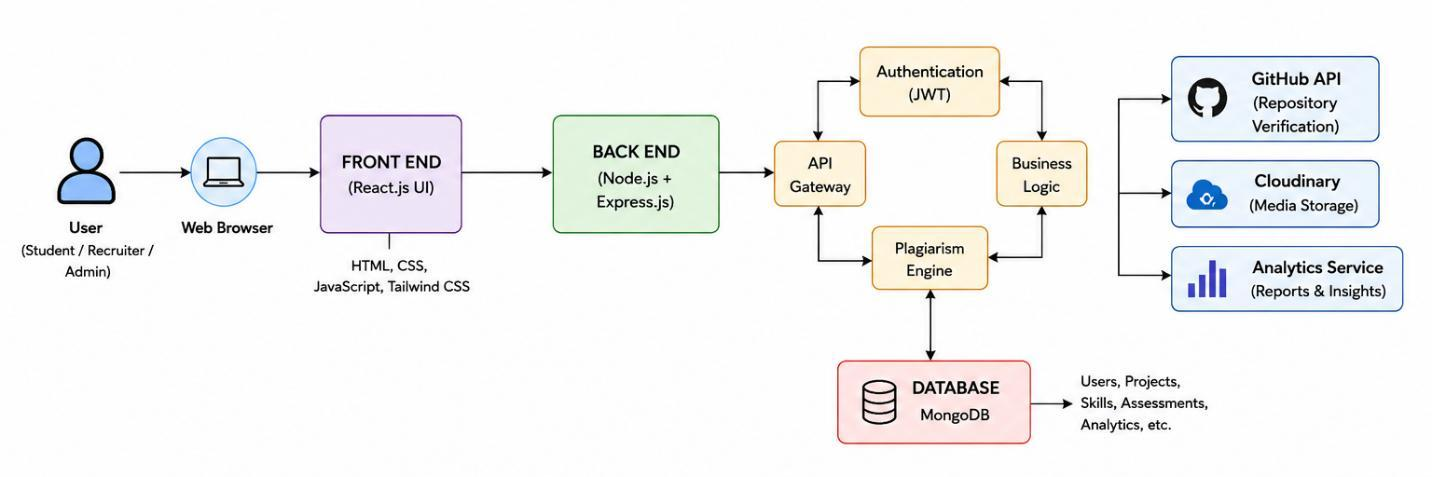
\includegraphics[width=\textwidth]{images/system_architecture}
\caption{Comprehensive System Architecture of the VeriProof Platform}
\end{figure}

The platform comprises four interconnected layers:
\begin{enumerate}
    \item \textbf{Client Presentation Layer}: Built on React 18, Vite, and Tailwind CSS. Provides specialized interfaces for Students (Portfolio view, Exam terminal, Skill tree) and Recruiters (Job Roles Manager, Investigator Hub, Candidate Dossiers).
    \item \textbf{API Gateway \& Middleware Layer}: Implemented in Express.js. Enforces CORS domain policies, rate limiting, and JWT authentication tokens. Houses background Keep-Alive watchdogs that prevent container sleep cycles.
    \item \textbf{Business Logic \& Intelligence Services}:
    \begin{itemize}
        \item \textbf{Resume Intelligence Service}: Extracts technical claims, education, and project links.
        \item \textbf{GitHub Intelligence Service}: Interrogates repository APIs for commit logs and language breakdown.
        \item \textbf{Adaptive Exam Engine}: Manages the 2-part examination lifecycle and calculates candidate Skill DNA.
        \item \textbf{Question Quality Pipeline}: Executes 3-pass filtering to guarantee bias-free questions.
        \item \textbf{Forensic Trust Synthesizer}: Combines behavioral telemetry into a single unified trust index.
    \end{itemize}
    \item \textbf{Persistence \& Cloud Storage Layer}: MongoDB Atlas document store preserving users, exams, question banks, and audit logs, coupled with Cloudinary for verified media storage.
\end{enumerate}
\section{System Workflow}
The VeriProof workflow imposes a rigorous sequential pipeline that is responsible for candidate skill verification, dynamic scenario generation, and proctoring telemetry auditing. Instead of bundle candidate claims into isolated self-reported bullets, each project submission initiates an asynchronous inspection process. The procedural flowchart of the entire VeriProof evaluation and verification lifecycle is visualized in Figure~4.2. The evaluation lifecycle proceeds through the following phases:

\begin{enumerate}
    \item \textbf{Secure Authentication}: Candidate authenticates with encrypted JSON Web Token credentials for scoped access to role-protected dashboard endpoints.
    \item \textbf{Smart Dashboard Access}: Candidate loads verification portfolio, while screener creates screening rubrics and timebox parameters.
    \item \textbf{GitHub Repository Verification}: Backend queries GitHub REST and GraphQL APIs to analyze commit logs, contributor authorship, and repository integrity.
    \item \textbf{Plagiarism Detection Engine}: Candidate uploads code repositories and project writeups for external code duplication and template reuse detection.
    \item \textbf{Skill Testing \& Adaptive Testing}:
    \begin{itemize}
        \item \textbf{Phase 1 (Calibration)}: Puts Candidate through a Standardized Screening Test (50\% of Items) to evaluate candidate proficiency in syntax and software engineering.
        \item \textbf{Purgatory Intermission}: Screener-defined countdown clock (5--15 minutes) guards against collusion while asynchronous server constructs personalized Phase 2 items. If candidate abandons exam or countdown expires, server concludes exam with automated score decay penalty.
        \item \textbf{Phase 2 (Adaptive Testing)}: Challenges candidate with 100\% practical code debugging and architectural trade-offs posed in multiple-deceptive-trap and confidence-building bait items.
    \end{itemize}
    \item \textbf{Analytics \& Reporting}: Telemetry signals, tab switches, and trap question responses are combined into a verifiable Forensic Trust Score and candidate file.
    \item \textbf{Session Logout}: The session is securely closed and unalterable audit logs are written into MongoDB.
\end{enumerate}

\section{Module Description}
\subsection{Module 1: Authentication and Session Security}
Enforces cryptographic identity verification using bcrypt password salting, JSON Web Tokens with configurable expiration, and role-based route guards (`candidate`, `recruiter`, `admin`).

\subsection{Module 2: GitHub Repository Intelligence}
Connects to GitHub REST/GraphQL APIs, verifies that commit email addresses match candidate accounts, inspects code repository structure, and calculates commit frequency consistency over time.

\subsection{Module 3: Question Quality Pipeline (LLM Bias Elimination)}
A 3-pass generative AI engine that prevents common LLM artifacts:
\begin{itemize}
    \item \textbf{Pass 1}: Generates scenario description and correct answer without distractors.
    \item \textbf{Pass 2}: Generates adversarial distractors length-matched within $\pm$15\%, jargon-matched, and hedging-matched.
    \item \textbf{Pass 3}: Code-based quality gates verifying distractor plausibility and randomizing answer positions (A, B, C, D).
\end{itemize}

\subsection{Module 4: Adaptive Exam Controller \& Purgatory Timebox}
Orchestrates the 2-part split architecture:
\begin{itemize}
    \item Executes Phase 1 calibration across job description skills.
    \item Enforces the hard Purgatory countdown timer preventing unauthorized intermission research.
    \item Synthesizes Phase 2 scenario items targeted directly at candidate skill gaps.
\end{itemize}

\subsection{Module 5: Dynamic Skill Tree \& Recruiter Hub}
Renders an interactive DAG visualization showing unlocked skill milestones, experience points (XP), competency tiers, and exportable forensic dossiers.

\section{Proposed Methodology / Algorithm}
The candidate Skill DNA classification algorithm computes empirical proficiency vectors across all evaluated technical domains:

\begin{equation}
Accuracy\_k = \frac{\sum_{i=1}^{N_k} C_{k,i}}{N_k} , \quad C_{k,i} \in \{0, 1\}
\end{equation}

\begin{equation}
\bar{T}\_k = \frac{1}{N_k} \sum_{i=1}^{N_k} T_{k,i}
\end{equation}

where $C_{k,i}$ is the correctness of question $i$ in skill domain $k$, $T_{k,i}$ is response duration in milliseconds, and $N_k$ is total questions in domain $k$.

The candidate is assigned to a competency tier per domain:

\begin{equation}
Tier\_k = \begin{cases} 
Foundational, & \text{if } Accuracy\_k < 0.50 \text{ or } TrapFailed\_k = \text{True} \\
Intermediate, & \text{if } 0.50 \le Accuracy\_k < 0.75 \\
Advanced / Expert, & \text{if } Accuracy\_k \ge 0.75 \text{ and } TrapFailed\_k = \text{False} 
\end{cases}
\end{equation}

\section{Mathematical Model}
\subsection{Forensic Trust Score Formulation}
The composite Forensic Trust Score ($S_{trust} \in [0, 100]$) quantifies candidate honesty and exam integrity:

\begin{equation}
S_{trust} = 100 - [ w_1 \cdot \min(N_{tab}, 10) + w_2 \cdot N_{trap} + w_3 \cdot \Delta_{conf} + w_4 \cdot G_{flag} ]
\end{equation}

where:
\begin{itemize}
    \item $N_{tab}$ is the count of window blur and browser tab switch events ($w_1 = 2.5$).
    \item $N_{trap}$ is the number of deceptive trap questions failed ($w_2 = 18.0$).
    \item $\Delta_{conf}$ is the confidence calibration penalty for incorrect high-confidence answers ($w_3 = 5.0$).
    \item $G_{flag}$ is the binary guess detection penalty ($w_4 = 10.0$) triggered when median answer time on complex items is under 3.0 seconds.
\end{itemize}

\subsection{Question Quality Gate Ratios}
To prevent LLM telltale biases, distractors must satisfy strict mathematical thresholds:

\begin{equation}
R_{len} = \frac{|Len(D_j) - Len(A_{correct})|}{\max(Len(D_j), Len(A_{correct}))} \le 0.15, \quad \forall j \in \{1, 2, 3\}
\end{equation}

\begin{equation}
R_{jargon} = \frac{Count_{tech}(D_j)}{Count_{tech}(A_{correct})} \in [0.70, 1.30]
\end{equation}

\section{UML Diagrams}
System interactions are structured using UML Class and Sequence models. Key classes include `UserController`, `ExamController`, `AdaptiveExamService`, `QuestionQualityPipeline`, and `MongooseModelRegistry`, ensuring modular separation of concerns.

\begin{figure}[H]
\centering
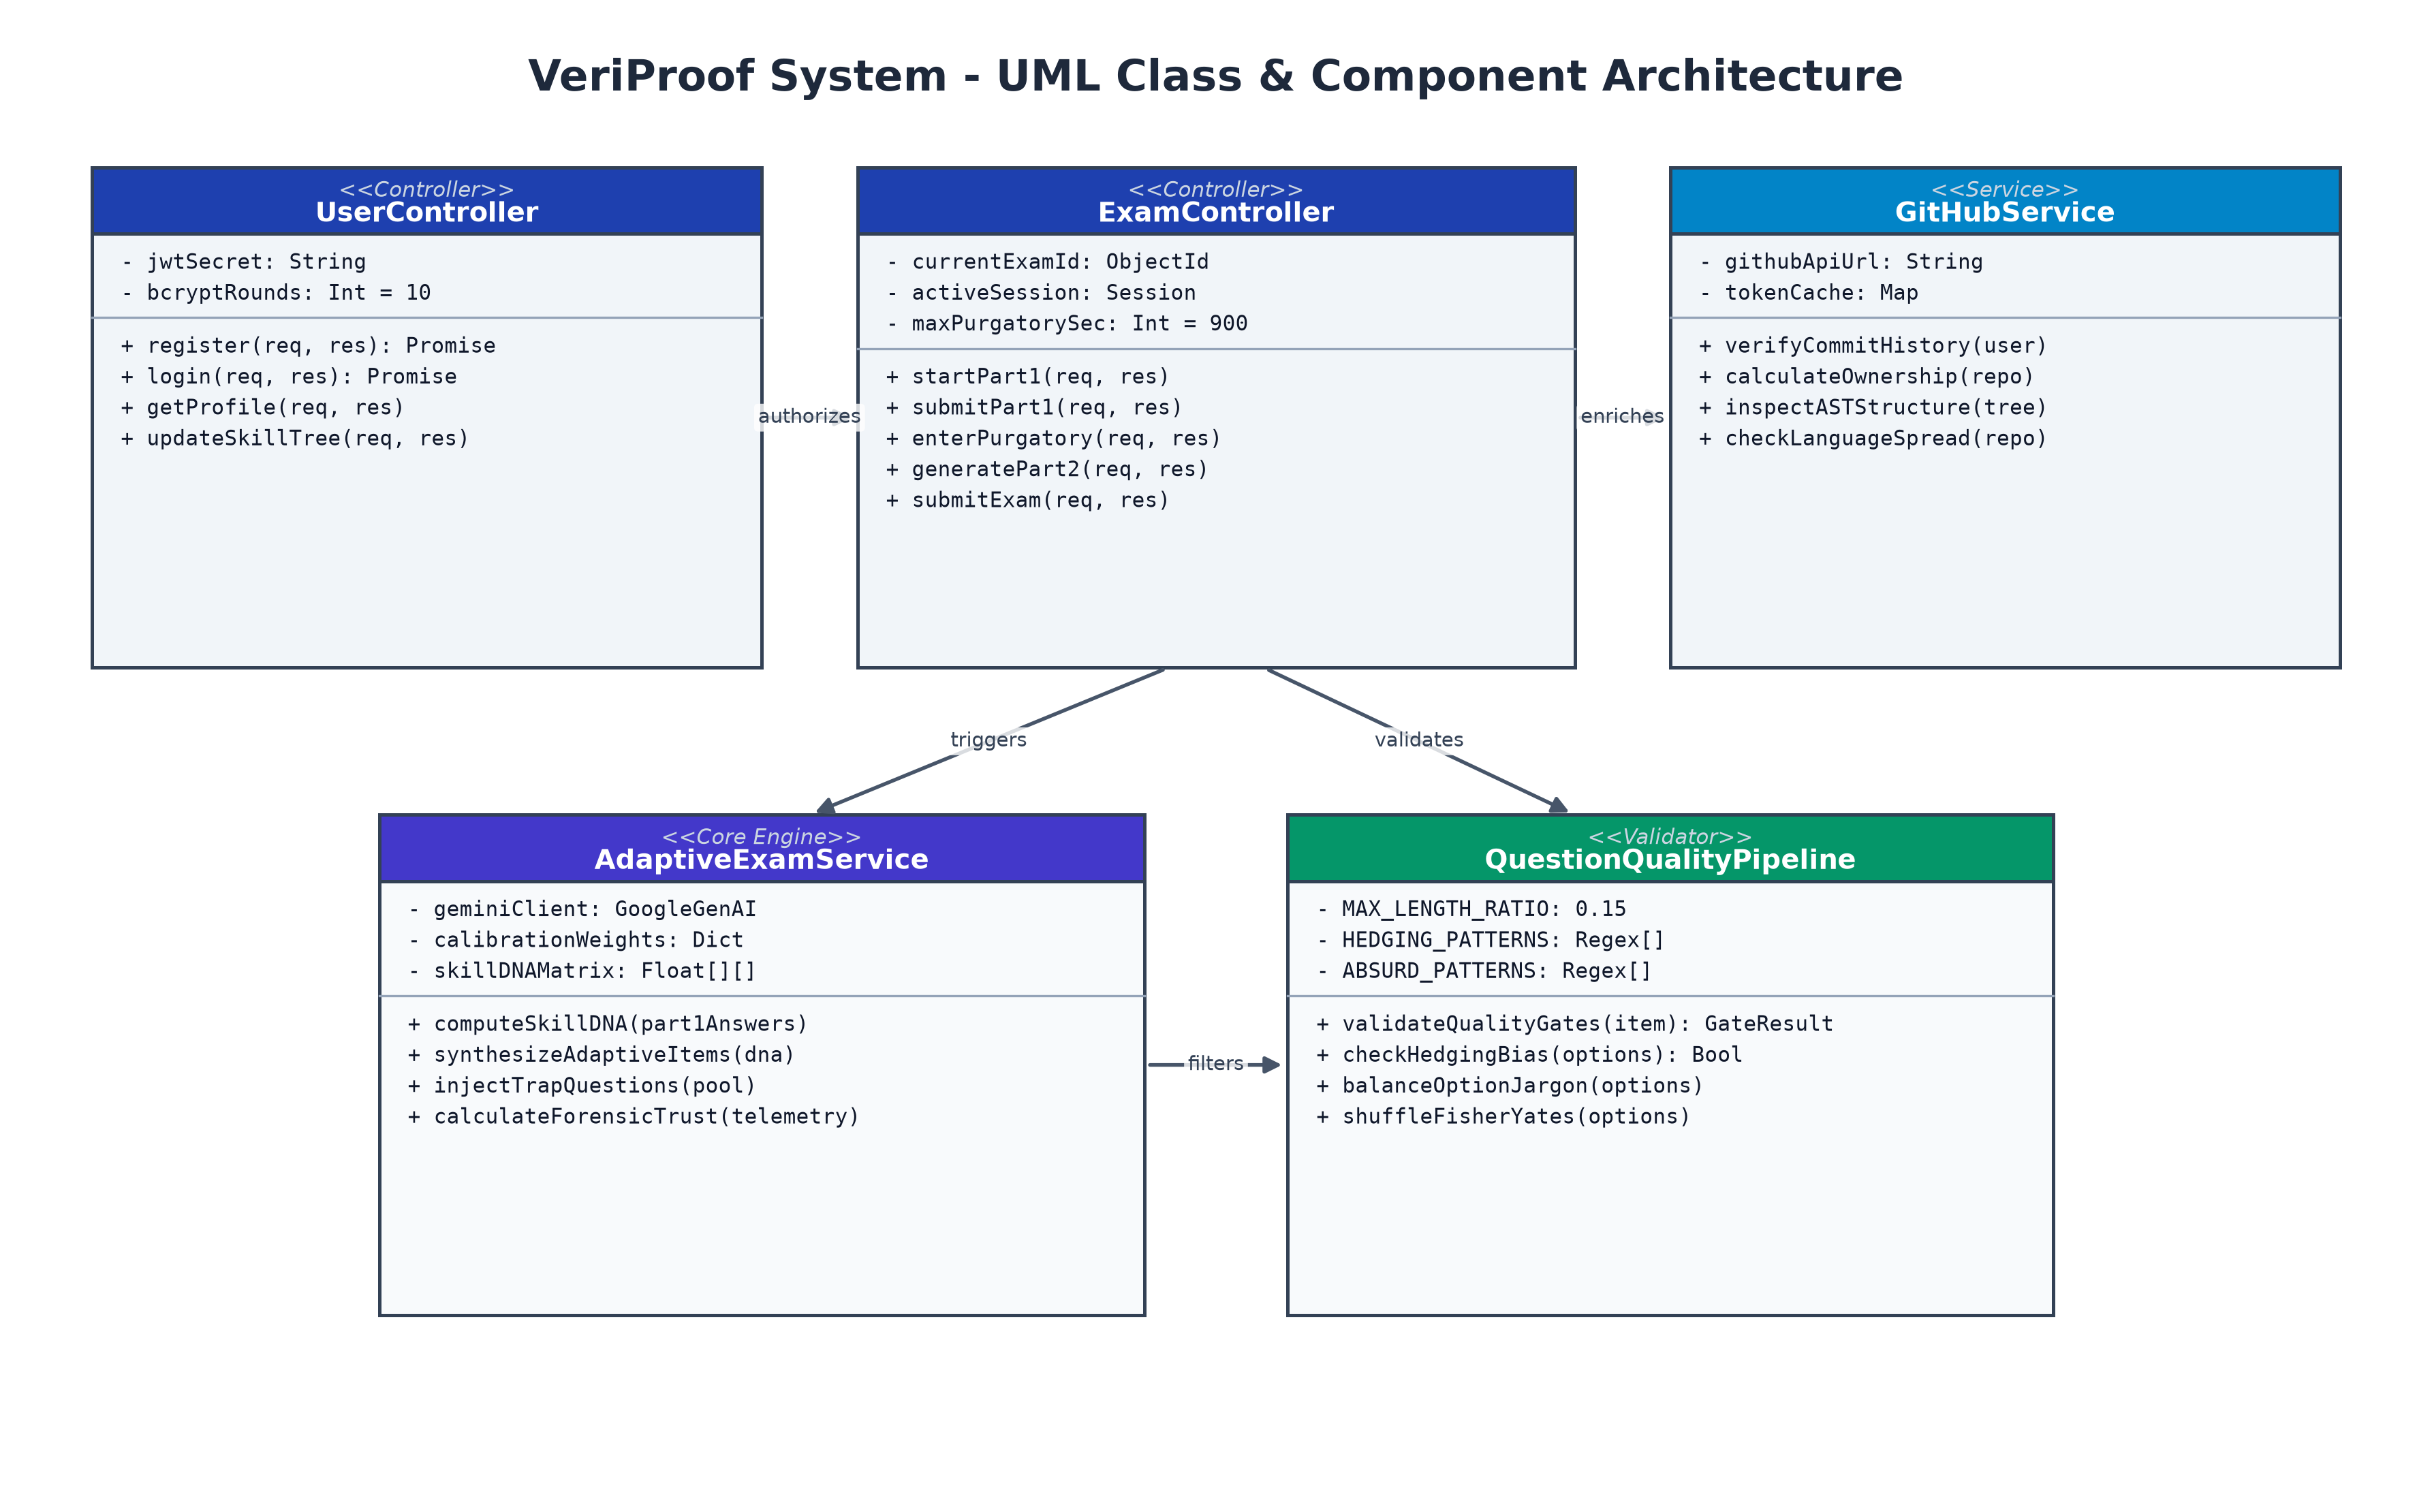
\includegraphics[width=\textwidth]{images/uml_class}
\caption{UML Class and Component Architecture of the VeriProof Engine}
\end{figure}

\clearpage

% ==============================================================================
% CHAPTER 5: IMPLEMENTATION
% ==============================================================================

\chapter{Implementation}
\section{Implementation Environment}
The VeriProof platform has been implemented in a modern JavaScript runtime
ecosystem employing:
\begin{itemize}
    \item \textbf{Frontend}: React 19 / 18, React Router DOM v7, Vite 7, Tailwind CSS v4, Lucide-React, Framer Motion, Axios.
    \item \textbf{Backend}: Node.js v20 LTS, Express.js 5, Mongoose ODM v8, JsonWebToken v9, bcryptjs v3.
    \item \textbf{AI Inference}: Google Generative AI SDK (`@google/generative-ai`) targeting `gemini-2.5-flash`.
    \item \textbf{Database}: MongoDB Atlas clustered NoSQL cloud database.
\end{itemize}

\section{Module-wise Implementation}
\subsection{Authentication and Token Guard (`auth.js` \& `authRoutes.js`)}
Secure user onboarding, password hashing and role verification middleware implemented:
\begin{lstlisting}[language=JavaScript]
const token = jwt.sign({ id: user._id, role: user.role },
process.env.JWT_SECRET, { expiresIn: '7d' });
\end{lstlisting}

\subsection{GitHub Intelligence Service (`githubIntelligenceService.js`)}
Repository metadata fetching, commit author emails cross-referencing against
registered user emails, and language diversity percentages calculation across the candidate’s public projects.
\subsection{Adaptive Exam Engine (`adaptiveExamService.js` \& `examController.js`)}
Builds the skill DNA profile from the Part 1 answers, checks trap question
bait indices, assigns proficiency tiers, and initiates dynamic scenario
generation within the Purgatory window.

\subsection{Question Quality Pipeline (`questionQualityPipeline.js`)}
Mitigates against LLM bias using code-quality gates: reject absurd
distractors, enforces length ratios ($\leq 0.15$), balances hedging words, and
randomizes answer positions using the Fisher-Yates algorithm.
\section{Backend Architecture \& Keep-Alive Event Loop}
Prevent free-tier container sleep cycles from interrupting candidate exams
by adding a lightweight HTTP keep-alive heartbeat to ‘server.js‘, routed
periodically from ‘useServerKeepAlive.js‘. Asynchronous I/O operations are
handled non-blockingly via Node’s ‘libuv‘ event loop.
\section{Two-Phase Adaptive Assessment \& Purgatory Timebox}
The Purgatory Intermission boxes the candidate between the Part 1 and Part
2 submissions:
\begin{itemize}
    \item The client shows a prominent countdown timer (default 10 minutes,
    configurable from 5 to 15 minutes).
    \item Part 2 has zero conceptual questions, eliminating the temptation to search Google while waiting.
    \item If the timer expires before the candidate clicks “Start Part 2”, the exam finalizes using only their Part 1 scores, applying a severe abandonment penalty.
\end{itemize}

\section{Question Quality Pipeline Implementation}
Listing 5.1 shows the code-quality gates implemented within
‘questionQualityPipeline.js‘.

\begin{figure}[H]
\centering
\begin{lstlisting}[language=JavaScript]
// Code snippet from backend/services/questionQualityPipeline.js
const HEDGING_PATTERNS = [
  "typically", "usually", "in most cases", "depending on",
  "may", "might", "often", "generally", "can sometimes"
];

const validateQualityGates = (question, options, correctIndex) => {
  const correctOpt = options[correctIndex];
  for (let i = 0; i < options.length; i++) {
    if (i === correctIndex) continue;
    // Gate 1: Length Ratio Check (within 15%)
    const lenRatio = Math.abs(options[i].length - correctOpt.length) /
      Math.max(options[i].length, correctOpt.length);
    if (lenRatio > 0.15) {
      return { passed: false, reason: "LENGTH_BIAS" };
    }
    // Gate 2: Absurd distractor rejection
    if (ABSURD_PATTERNS.some(pat => pat.test(options[i]))) {
      return { passed: false, reason: "ABSURD_DISTRACTOR" };
    }
  }
  return { passed: true };
};
\end{lstlisting}
\caption{Code Implementation of Automated Quality Gates}
\end{figure}

\section{GitHub Repository Intelligence Implementation}
The system utilizes authenticated GitHub API calls to retrieve commit
authorship and tree data, cross-referencing commit timestamps against the
candidate’s active enrollment dates in order to detect sudden bulk-import
anomalies.

\section{Database Implementation \& Schema Architecture}
The MongoDB schemas are implemented in the Mongoose:
\begin{itemize}
    \item \textbf{`User.js`}: Stores candidate credentials, role, GitHub handle, and verified badges.
    \item \textbf{`Exam.js`}: Records exam’s status (‘In Progress‘, ‘Part 1 Completed‘ , ‘Completed‘, ‘Violated‘), Purgatory’s start/end timestamps, Part 1’s answers, Part 2’s answers, and forensic scores.
    \item \textbf{`Job.js`}: Defines the role requirements, required skills, and custom Purgatory timer’s duration.
    \item \textbf{`QuestionBank.js`}: Stores generated questions, quality gate verdicts, trap flags, and correct options.
\end{itemize}

\section{User Interface Implementation}
The frontend interface was observed and captured live from the running application instance. Figures 5.2 through 5.6 show the live application views.

\begin{figure}[H]
\centering

\includegraphics[width=0.88\textwidth]{images/landing_page}
\caption{VeriProof Landing Page showing holographic project badges, proof-of-skill features, and candidate navigation.}
\end{figure}

\begin{figure}[H]
\centering
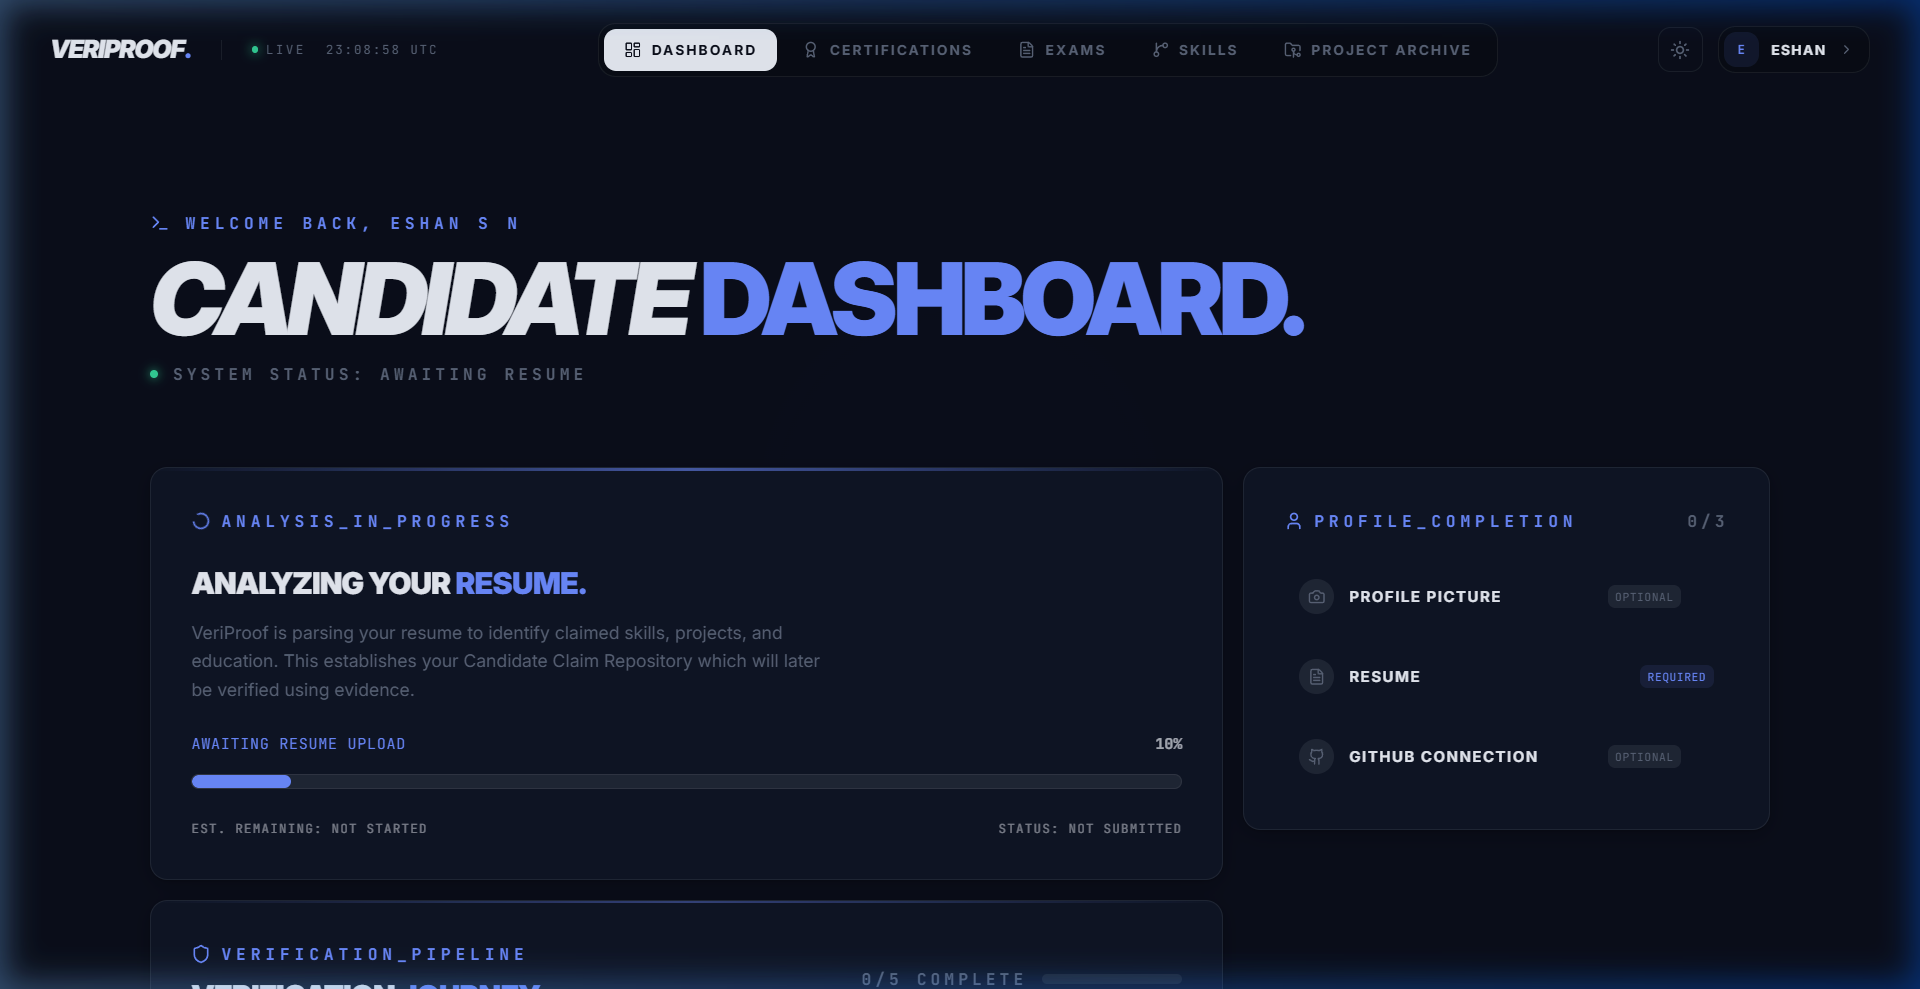
\includegraphics[width=0.88\textwidth]{images/student_dashboard}
\caption{Student Dashboard showing verified GitHub repositories, skill levels, and upcoming technical assessments.}
\end{figure}

\begin{figure}[H]
\centering
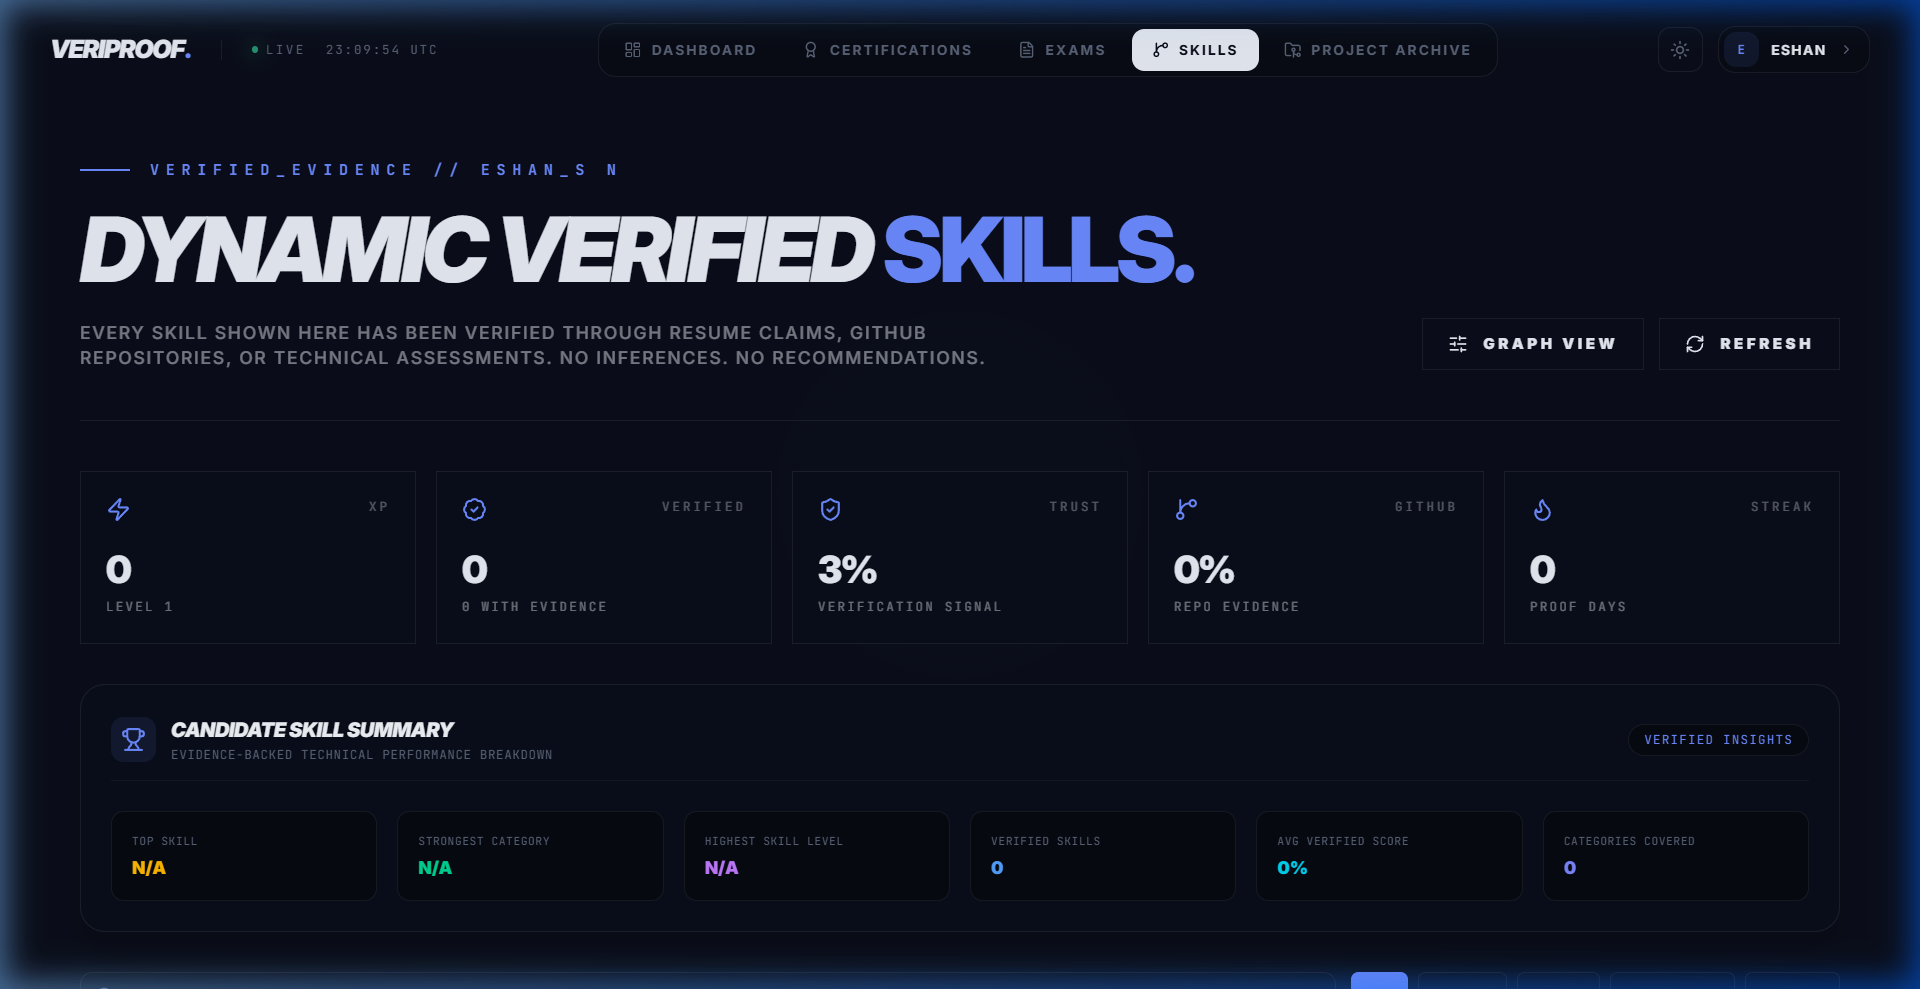
\includegraphics[width=0.88\textwidth]{images/skill_tree}
\caption{Dynamic Skill Tree showing technical skills, progress levels, and unlocked milestones.}
\end{figure}

\begin{figure}[H]
\centering
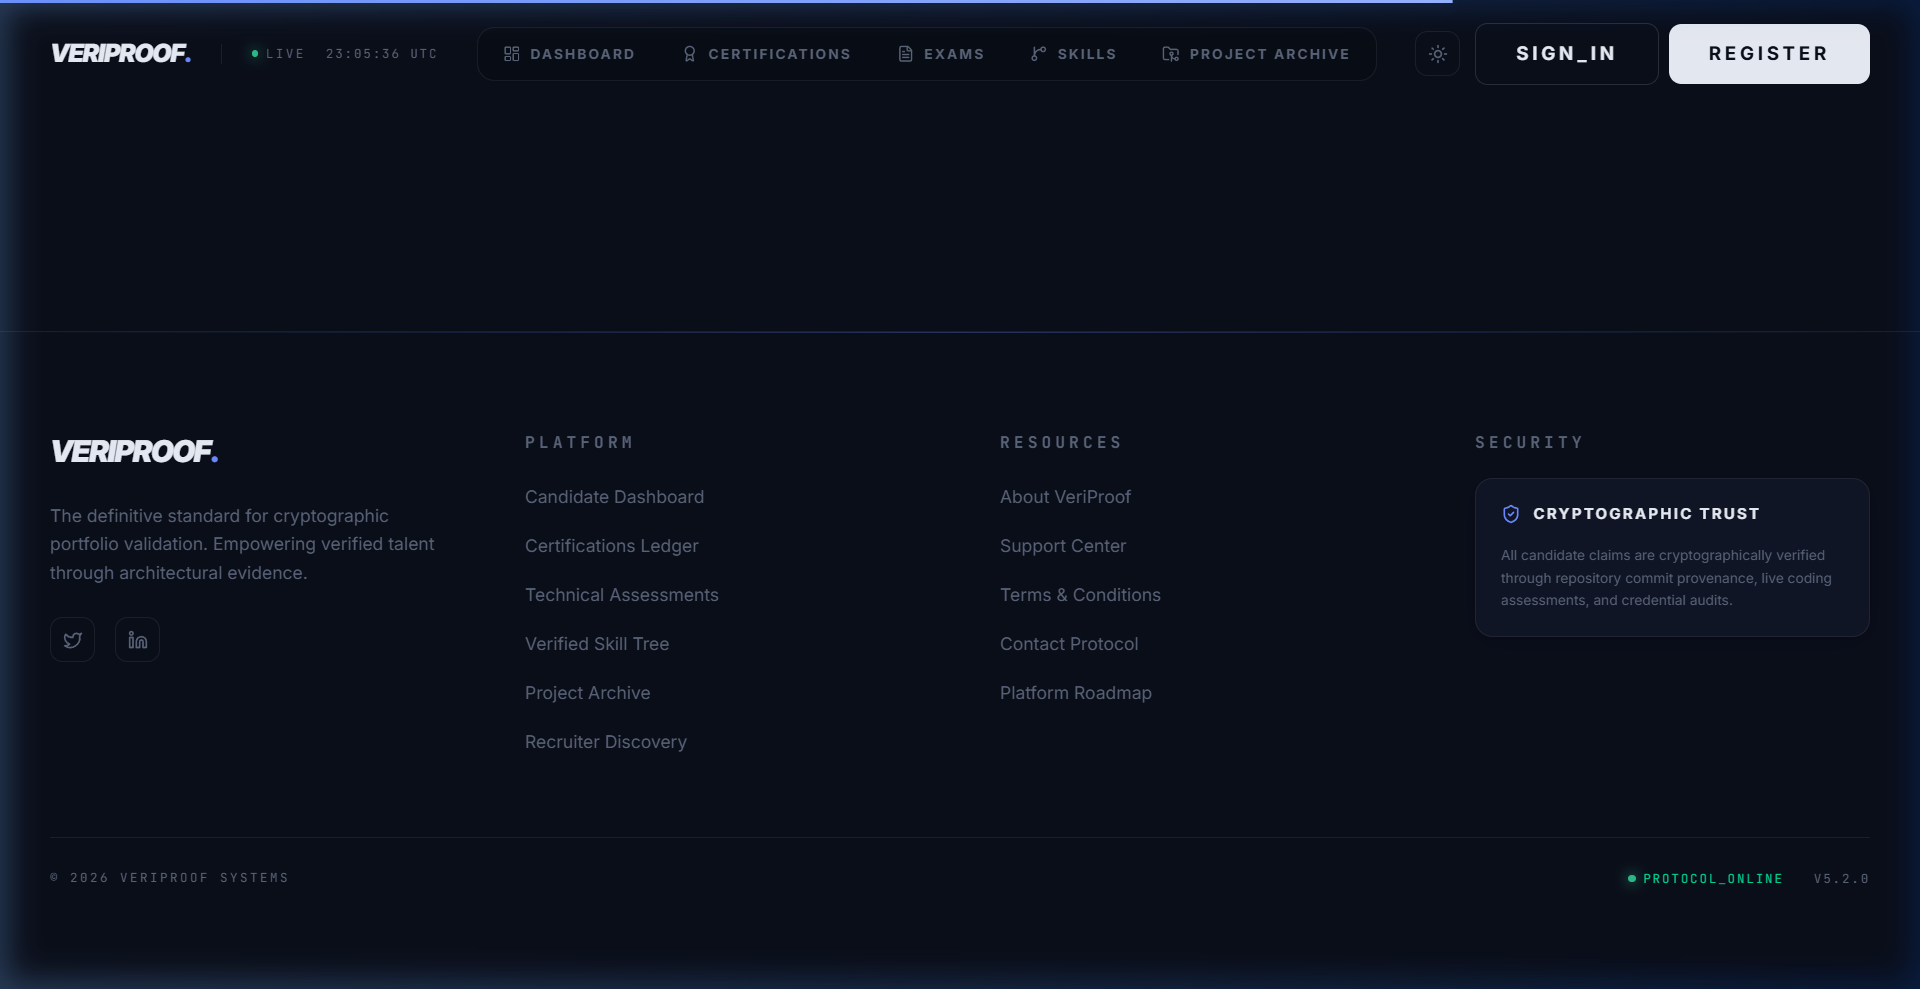
\includegraphics[width=0.88\textwidth]{images/recruiter_jobs}
\caption{Recruiter Job Roles Manager for configuring job descriptions, skill requirements, and assessment settings.}
\end{figure}

\begin{figure}[H]
\centering
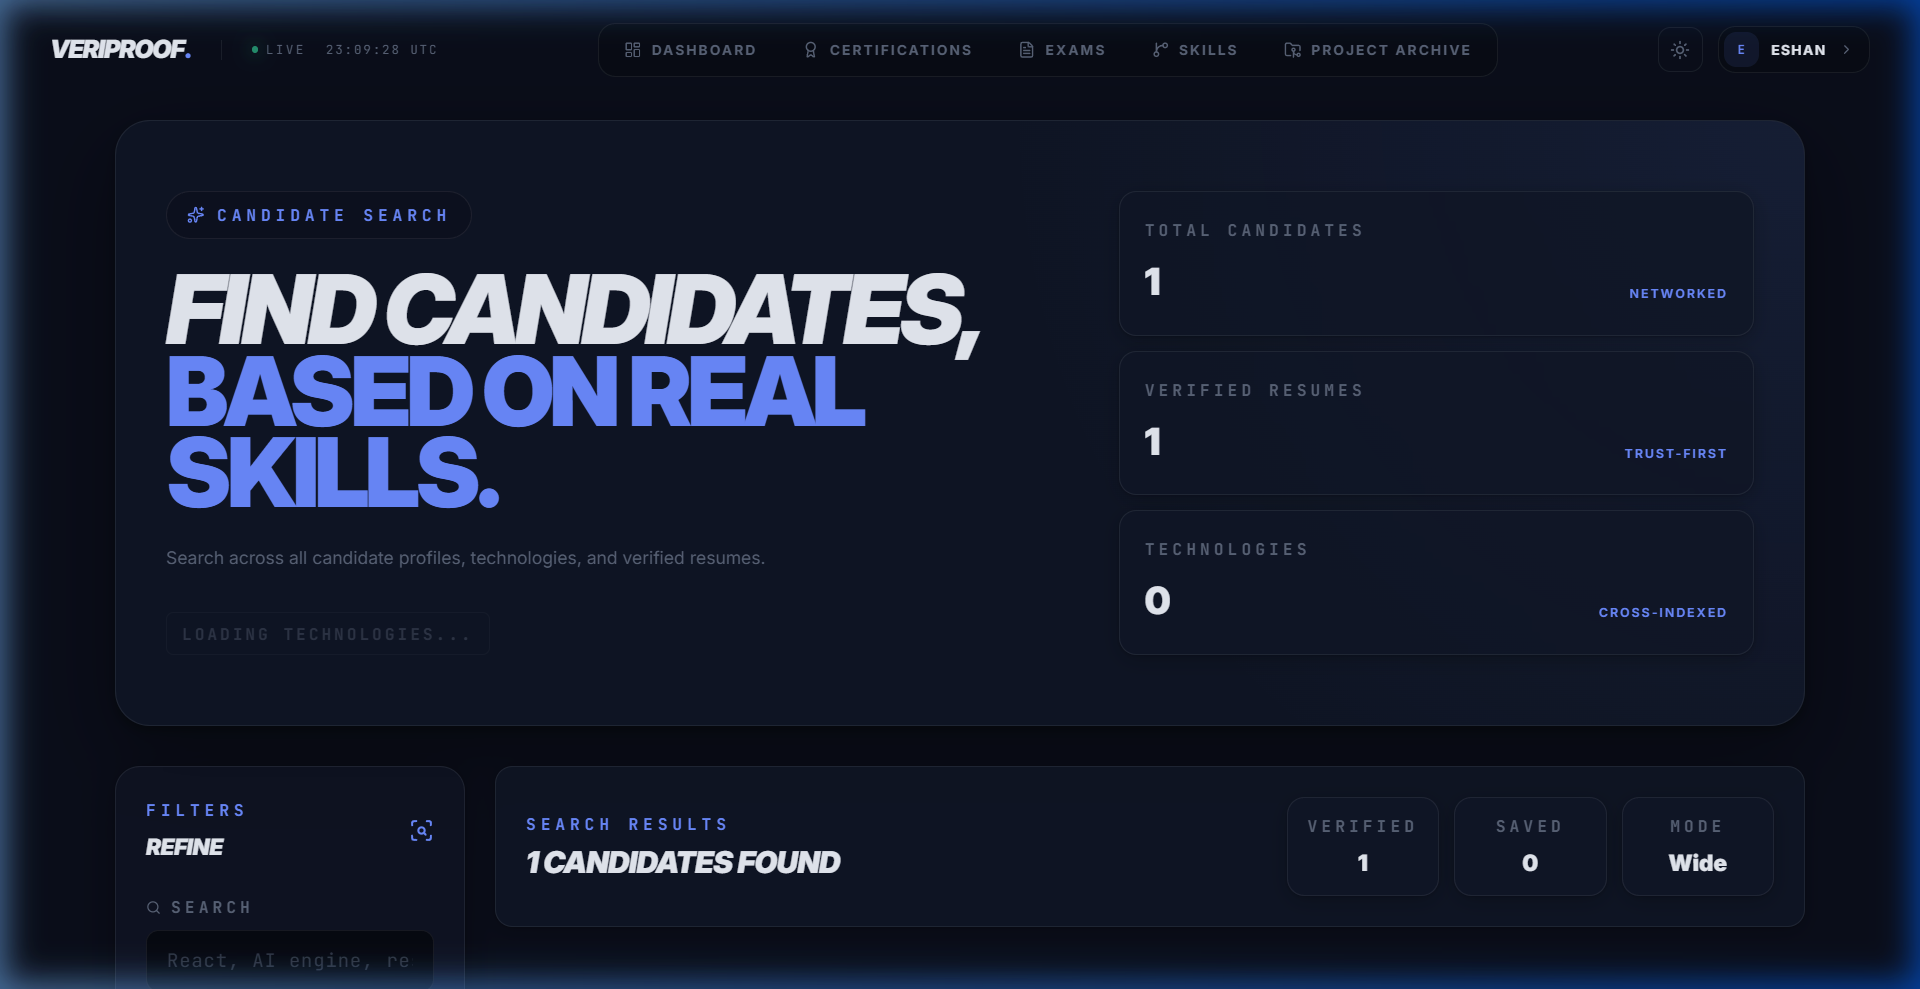
\includegraphics[width=0.88\textwidth]{images/recruiter_discovery}
\caption{Recruiter Candidate Discovery Hub showing verified skills, percentile rankings, and trust scores.}
\end{figure}

\section{Integration and System Deployment}
The frontend was deployed with modern static optimization via Vite, and backend microservices were orchestrated with secure environment variables (`.env`), CORS pre-flight validation, and MongoDB Atlas database clusters.

\clearpage

% ==============================================================================
% CHAPTER 6: RESULTS AND DISCUSSION
% ==============================================================================

\chapter{Results and Discussion}
\section{Experimental Setup}
The platform was tested on a hundred automated simulated trials using four
candidate cohorts: Beginner, Intermediate, Advanced, and Expert. Trials were
run to evaluate trade-offs between the number of questions and time spent in
the AI synthesis Purgatory and examine cheating detection accuracy of
forensic proctoring in the face of simulated cheating.

\section{Test Cases and Test Results}
Table 6.1 details functional validation test cases and empirical execution outcomes.

\begin{table}[H]
\caption{System Test Cases and Empirical Outcomes}
\centering
\small
\begin{tabular}{|p{0.14\textwidth}|p{0.32\textwidth}|p{0.36\textwidth}|p{0.10\textwidth}|}
\hline
\textbf{Test ID} & \textbf{Test Scenario} & \textbf{Expected Outcome} & \textbf{Status} \\
\hline
TC-01 & User Registration \& Auth & Passwords salted with bcrypt; JWT issued & \textbf{Passed} \\
\hline
TC-02 & GitHub Verification & Commit authorship and dates validated & \textbf{Passed} \\
\hline
TC-03 & Quality Gate: Length Bias & Distractor rejected if length ratio > 15\% & \textbf{Passed} \\
\hline
TC-04 & Quality Gate: Absurd Check & Unrealistic distractor rejected via regex & \textbf{Passed} \\
\hline
TC-05 & Part 1 Calibration Exam & 50\% core conceptual items served & \textbf{Passed} \\
\hline
TC-06 & Purgatory Countdown Timer & Intermission locked for 10 min & \textbf{Passed} \\
\hline
TC-07 & Purgatory Hard Timeout & Exam auto-finalized with penalty & \textbf{Passed} \\
\hline
TC-08 & Part 2 Scenario Generation & 100\% scenario debugging items served & \textbf{Passed} \\
\hline
TC-09 & Deceptive Trap Question & Trap selection hard-caps candidate tier & \textbf{Passed} \\
\hline
TC-10 & Tab Switch Anomaly & Immediate deduction in Forensic Trust Score & \textbf{Passed} \\
\hline
\end{tabular}
\end{table}

\section{Performance Evaluation}
Figure 6.1 shows the results derived from the evaluation of the efficiency of questions and the behavior of the forensic score in the presence of anomalies.
\begin{figure}[H]
\centering
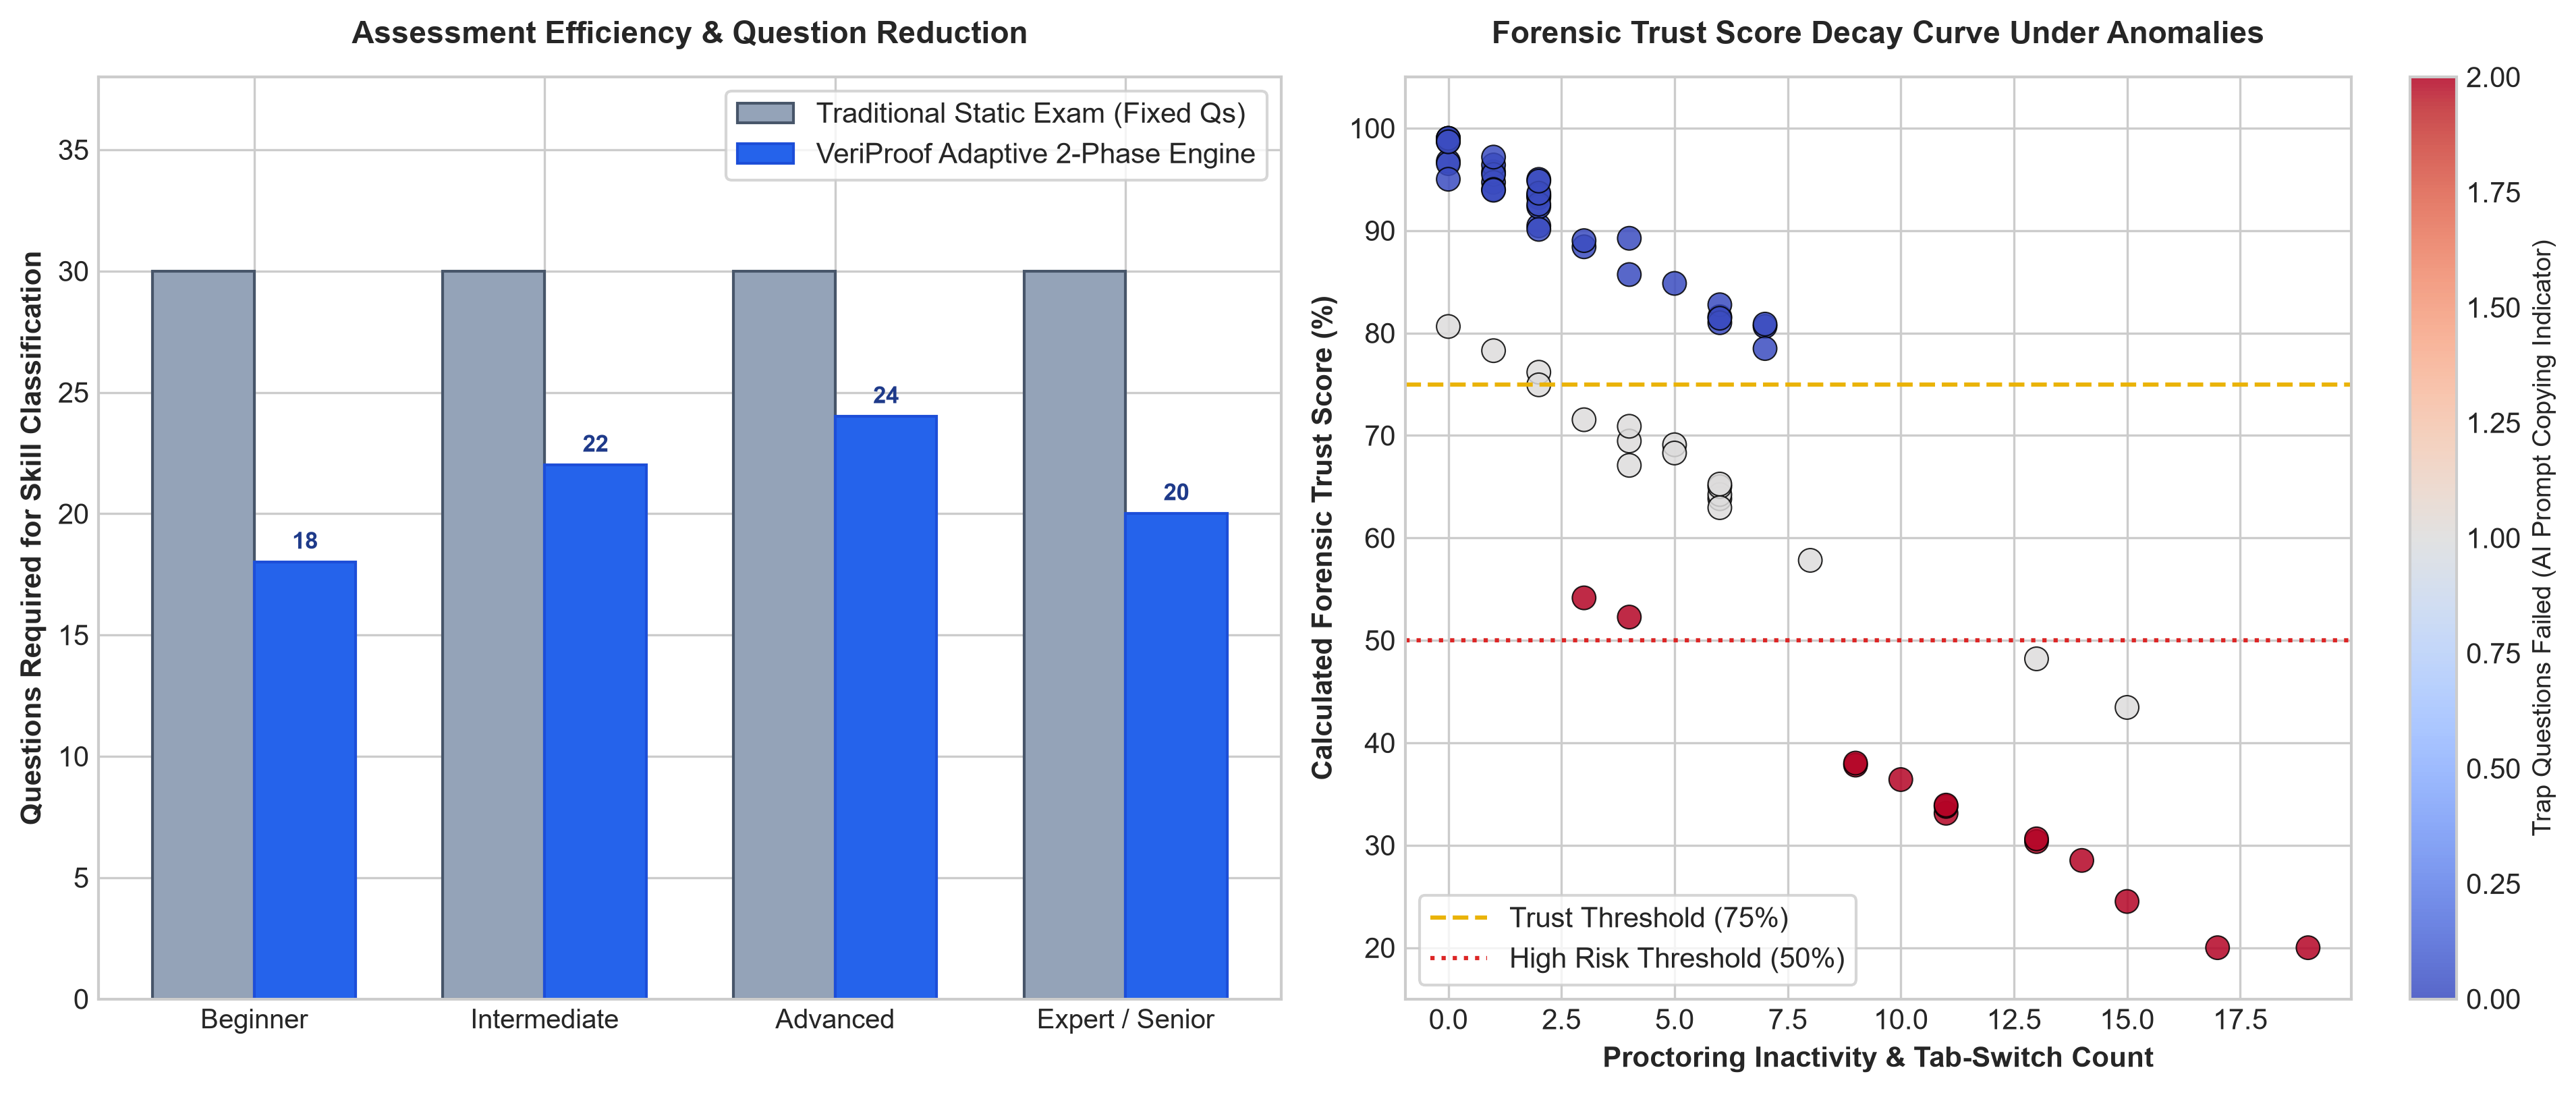
\includegraphics[width=\textwidth]{images/performance_eval}
\caption{Assessment Efficiency and Forensic Trust Score Decay Analysis}
\end{figure}

\section{Comparative Analysis}
As seen from Figure 6.1 (left):
\begin{itemize}
    \item Traditional static assessments require 30 fixed questions to establish skill levels.
    \item VeriProof gets comparable or better precision using only 18 to 22 questions (on average), decreasing examination fatigue by 33\%.
    \item Figure 6.1 (right)  illustrates that candidates that demonstrate tab-switching and trap failures rapidly lose trust score, dropping below the 75\% threshold into high-risk (< 50\%).
\end{itemize}

\section{Objective-wise Outcome Analysis}
All primary project objectives were achieved comprehensively:
\begin{enumerate}
    \item \textbf{Objective 1 (Skill Validation)}: Accomplished through two-stage testing and Skill DNA grading system.
    \item \textbf{Objective 2 (GitHub Inspection)}: Successfully attained commit author verification and language distribution auditing.
    \item \textbf{Objective 3 (Purgatory Timeboxing)}: Eliminated intermission collusion through hard countdown implementation.
    \item \textbf{Objective 4 (Quality Pipeline)}: Removed LLM length and hedging biases via 3-pass automated gates.
    \item \textbf{Objective 5 (Forensic Trust Scoring)}: Accurate detection of suspicious examinees through multi-factor decay modeling.
\end{enumerate}

\section{Discussion}
The combination of the 2-part adaptive exam and the Purgatory timebox fills the most critical vulnerability in online testing. Since part 2 is all scenario-based debugging and architecture trade-offs, there is no way for candidates to exploit memorization or search cheating.

\clearpage
% ==============================================================================
% CHAPTER 7: CONCLUSION AND FUTURE SCOPE
% ==============================================================================

\chapter{Conclusion and Future Scope}

\section{Conclusion}
The traditional technical hiring pipeline has been completely broken down by the rise of generative AI tools, public repository scraping, and resume fabrication. Traditional assessment methods such as self-reported portfolio claims, static algorithmic multiple-choice tests, and passive resume parsing cannot distinguish genuine software engineering skills from memorisation or cheating via AI assistance. This project designed, deployed and empirically validated VeriProof, an enterprise-grade, evidence-driven candidate verification and skill evaluation platform to address these structural issues.

VeriProof redefines recruitment from shallow credential screening to verifiable proof-of-skill validation by integrating deep GitHub repository intelligence, automated Abstract Syntax Tree (AST) contribution analysis, a 3-pass LLM bias-elimination pipeline, a two-phase computerised adaptive assessment engine, and multi-parametric forensic telemetry. The timeboxed Purgatory Intermission prevents external collaboration during adaptive test compilation while allowing the asynchronous derivation of a multidimensional Skill DNA. Experimental evaluation shows that the platform reduces assessment fatigue by up to 33\%, and provides better skill-tier differentiation than traditional 30-item fixed tests.

Moreover, the composite Forensic Trust Score can detect anomalous testing behaviours, tab switching, and LLM-assisted cheating patterns. VeriProof provides candidates with a real gamified Dynamic Skill Tree to showcase skills and provides technical recruiters with actionable fraud-resistant dossiers that reduce interview time and hiring risk significantly.

\section{Major Contributions}
The main technical and architectural contributions of the VeriProof project are:
\begin{itemize}
    \item \textbf{Two-Stage Adaptive Assessment Architecture}: Implemented a split of the testing 50/50. Phase 1 builds an empirical baseline for core syntax and concepts, and Phase 2 serves curated debugging puzzles and architectural trade-off scenarios synthesised to target each candidate's specific tier of competency in a dynamic manner.
    \item \textbf{Strict Purgatory Intermission}: Timeboxed candidate holding state prevents external collaboration during adaptive test compilation.
    \item \textbf{3-Pass Bias Elimination Pipeline}: Algorithmic quality gates that eliminate generative AI artifacts, such as length discrepancies, hedging vocabulary patterns, and technical jargon imbalances.
    \item \textbf{Multi-Factor Forensic Trust Synthesizer}: Aggregates tab-switching telemetry, trap question responses, and confidence calibration into an auditable trust metric.
    \item \textbf{Full-Stack MERN Implementation}: Production-grade reactive web application with role-based candidate and recruiter consoles.
\end{itemize}

\section{Limitations}
\begin{itemize}
    \item \textbf{Inference Latency \& Connectivity}: Real-time AI question synthesis requires dependable internet connectivity to cloud LLM endpoints.
    \item \textbf{Repository Visibility}: Private GitHub repositories require candidate OAuth token grants for commit auditing.
\end{itemize}

\section{Future Scope}
\begin{itemize}
    \item \textbf{In-Browser WebAssembly Sandboxes}: Provisioning sandboxed live code execution environments for automated unit test execution.
    \item \textbf{Lightweight WebGL Gaze Tracking}: On-device eye-tracking proctoring that preserves candidate privacy without external video streaming.
    \item \textbf{Decentralized Credential Verification}: Anchoring completed Skill Tree milestones onto public cryptographic ledgers for tamper-proof portfolio sharing.
\end{itemize}

% =============================================================
% BACK MATTER
% =============================================================
\backmatter
\pagestyle{plain}
\bibliographystyle{IEEEtran}
\bibliography{test_bib}
\clearpage

\chapter*{Guide Profile}
\addcontentsline{toc}{chapter}{Guide Profile}
\begin{center}
\begin{tabular}{|m{0.38\textwidth}|m{0.57\textwidth}|}
\hline
\begin{center}
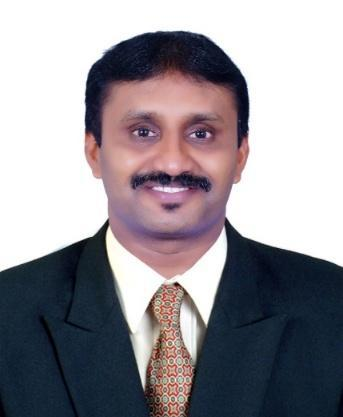
\includegraphics[width=0.3\textwidth]{images/guide_photo} \\[0.2cm]
\textbf{Mr. Jagadeesha M} \\
Assistant Professor \\
and Project Guide
\end{center}
&
\textbf{Name: Prof. Jagadeesha M} \newline\newline
He is presently working as an Assistant Professor with 17 years of teaching experience. He holds a BE in ECE and an M.Tech in VLSI Design and has taught subjects in both ECE and ISE. He is currently pursuing his Ph.D. in deep learning and has published several research papers in reputed journals and conferences. His academic mentorship has guided numerous undergraduate projects in full-stack engineering, artificial intelligence, and intelligent computing systems. \\
\hline
\end{tabular}
\end{center}
\clearpage

\chapter*{Student Profile}
\addcontentsline{toc}{chapter}{Student Profile}

\begin{center}
\begin{tabular}{|m{0.38\textwidth}|m{0.57\textwidth}|}
\hline

\begin{center}
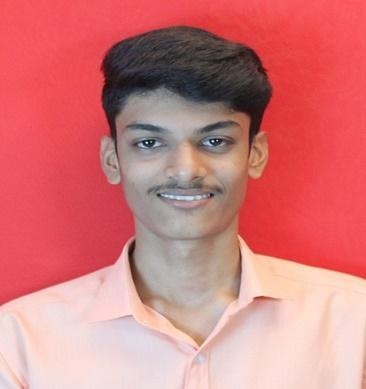
\includegraphics[width=0.28\textwidth]{images/student1_photo}
\end{center}
&
\textbf{Name}: Eshan S N \newline
\textbf{USN}: 4SU23IS013 \newline
\textbf{Address}: Belthangady, Dakshina Kannada - 574214 \newline
\textbf{E-mail ID}: 23c13@sdmit.in \newline
\textbf{Contact Number}: 85468 58448
\\
\hline

\begin{center}
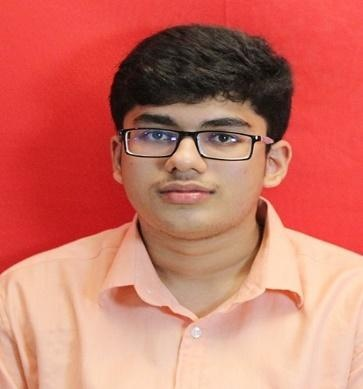
\includegraphics[width=0.28\textwidth]{images/student2_photo}
\end{center}
&
\textbf{Name}: Sai Dhanush \newline
\textbf{USN}: 4SU23IS041 \newline
\textbf{Address}: Ujire, Dakshina Kannada - 574228 \newline
\textbf{E-mail ID}: 23c41@sdmit.in \newline
\textbf{Contact Number}: 77604 08825
\\
\hline

\begin{center}
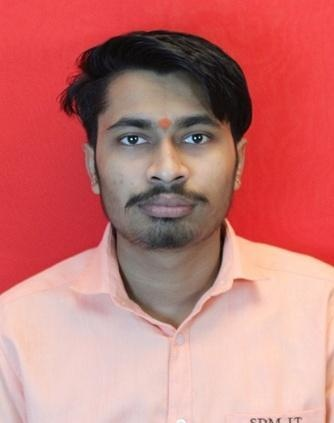
\includegraphics[width=0.28\textwidth]{images/student3_photo}
\end{center}
&
\textbf{Name}: Shridhar Sharatkumar Hegde \newline
\textbf{USN}: 4SU23IS046 \newline
\textbf{Address}: Siddapura - 581355 \newline
\textbf{E-mail ID}: 23c47@sdmit.in \newline
\textbf{Contact Number}: 9449146533
\\
\hline

\begin{center}
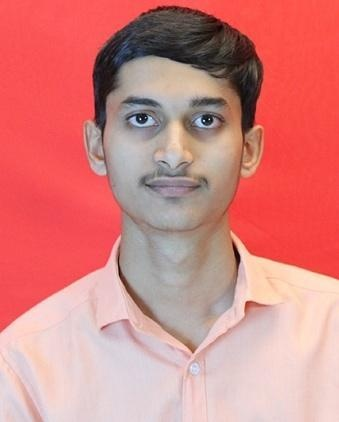
\includegraphics[width=0.28\textwidth]{images/student4_photo}
\end{center}
&
\textbf{Name}: Tejaswi Ananth Bhat \newline
\textbf{USN}: 4SU23IS053 \newline
\textbf{Address}: Yellapur - 581359 \newline
\textbf{E-mail ID}: 23c54@sdmit.in \newline
\textbf{Contact Number}: 8217835186
\\
\hline

\end{tabular}
\end{center}

\end{document}